\documentclass[11pt,a4paper]{article}

\usepackage[margin=1in]{geometry}
\usepackage{graphicx}
\usepackage{booktabs}
\usepackage{hyperref}
\usepackage{amsmath}
\usepackage{xcolor}
\usepackage{float}
\usepackage{subcaption}
\usepackage{enumitem}

\newcommand{\todo}[1]{{\color{red}\textbf{[TODO: #1]}}}

% Auto-generated data macros from benchmark results.
% Regenerate: cd task1 && python3 generate_data.py
% AUTO-GENERATED by generate_data.py -- do not edit by hand
% Re-run:  cd task1 && python3 generate_data.py


% === Unroll speedups ===
\newcommand{\unrollUnrollOxKthreeFtwelve}{2.89x}
\newcommand{\unrollUnrollOxKthreeTtwentyfour}{3.19x}
\newcommand{\unrollUnrollOxKthreeTfortyeight}{2.94x}
\newcommand{\unrollUnrollOxKthreeFninetysix}{2.98x}
\newcommand{\unrollUnrollOxKthreeEonetwelve}{2.93x}
\newcommand{\unrollUnrollKxKthreeFtwelve}{0.65x}
\newcommand{\unrollUnrollKxKthreeTtwentyfour}{0.65x}
\newcommand{\unrollUnrollKxKthreeTfortyeight}{0.61x}
\newcommand{\unrollUnrollKxKthreeFninetysix}{0.62x}
\newcommand{\unrollUnrollKxKthreeEonetwelve}{0.63x}
\newcommand{\unrollUnrollKyKthreeFtwelve}{0.85x}
\newcommand{\unrollUnrollKyKthreeTtwentyfour}{0.84x}
\newcommand{\unrollUnrollKyKthreeTfortyeight}{0.84x}
\newcommand{\unrollUnrollKyKthreeFninetysix}{0.88x}
\newcommand{\unrollUnrollKyKthreeEonetwelve}{0.87x}
\newcommand{\unrollUnrollOxOyKthreeFtwelve}{2.85x}
\newcommand{\unrollUnrollOxOyKthreeTtwentyfour}{2.67x}
\newcommand{\unrollUnrollOxOyKthreeTfortyeight}{2.61x}
\newcommand{\unrollUnrollOxOyKthreeFninetysix}{2.57x}
\newcommand{\unrollUnrollOxOyKthreeEonetwelve}{2.71x}
\newcommand{\unrollReordOxKthreeFtwelve}{1.68x}
\newcommand{\unrollReordOxKthreeTtwentyfour}{1.09x}
\newcommand{\unrollReordOxKthreeTfortyeight}{0.61x}
\newcommand{\unrollReordOxKthreeFninetysix}{0.59x}
\newcommand{\unrollReordOxKthreeEonetwelve}{0.54x}
\newcommand{\unrollReordOyKthreeFtwelve}{1.26x}
\newcommand{\unrollReordOyKthreeTtwentyfour}{0.70x}
\newcommand{\unrollReordOyKthreeTfortyeight}{0.55x}
\newcommand{\unrollReordOyKthreeFninetysix}{0.49x}
\newcommand{\unrollReordOyKthreeEonetwelve}{0.49x}
\newcommand{\unrollReordOxOyKthreeFtwelve}{1.31x}
\newcommand{\unrollReordOxOyKthreeTtwentyfour}{0.89x}
\newcommand{\unrollReordOxOyKthreeTfortyeight}{0.54x}
\newcommand{\unrollReordOxOyKthreeFninetysix}{0.53x}
\newcommand{\unrollReordOxOyKthreeEonetwelve}{0.53x}
\newcommand{\unrollReordKxKthreeFtwelve}{1.33x}
\newcommand{\unrollReordKxKthreeTtwentyfour}{0.94x}
\newcommand{\unrollReordKxKthreeTfortyeight}{0.49x}
\newcommand{\unrollReordKxKthreeFninetysix}{0.45x}
\newcommand{\unrollReordKxKthreeEonetwelve}{0.50x}
\newcommand{\unrollUnrollOxKfiveFtwelve}{2.62x}
\newcommand{\unrollUnrollOxKfiveTtwentyfour}{2.66x}
\newcommand{\unrollUnrollOxKfiveTfortyeight}{2.66x}
\newcommand{\unrollUnrollOxKfiveFninetysix}{2.61x}
\newcommand{\unrollUnrollOxKfiveEonetwelve}{2.64x}
\newcommand{\unrollUnrollKxKfiveFtwelve}{1.09x}
\newcommand{\unrollUnrollKxKfiveTtwentyfour}{1.12x}
\newcommand{\unrollUnrollKxKfiveTfortyeight}{1.10x}
\newcommand{\unrollUnrollKxKfiveFninetysix}{1.08x}
\newcommand{\unrollUnrollKxKfiveEonetwelve}{1.11x}
\newcommand{\unrollUnrollKyKfiveFtwelve}{1.01x}
\newcommand{\unrollUnrollKyKfiveTtwentyfour}{1.00x}
\newcommand{\unrollUnrollKyKfiveTfortyeight}{1.00x}
\newcommand{\unrollUnrollKyKfiveFninetysix}{0.99x}
\newcommand{\unrollUnrollKyKfiveEonetwelve}{1.00x}
\newcommand{\unrollUnrollOxOyKfiveFtwelve}{2.83x}
\newcommand{\unrollUnrollOxOyKfiveTtwentyfour}{2.73x}
\newcommand{\unrollUnrollOxOyKfiveTfortyeight}{2.70x}
\newcommand{\unrollUnrollOxOyKfiveFninetysix}{2.71x}
\newcommand{\unrollUnrollOxOyKfiveEonetwelve}{2.69x}
\newcommand{\unrollReordOxKfiveFtwelve}{1.46x}
\newcommand{\unrollReordOxKfiveTtwentyfour}{1.04x}
\newcommand{\unrollReordOxKfiveTfortyeight}{0.61x}
\newcommand{\unrollReordOxKfiveFninetysix}{0.51x}
\newcommand{\unrollReordOxKfiveEonetwelve}{0.49x}
\newcommand{\unrollReordOyKfiveFtwelve}{1.15x}
\newcommand{\unrollReordOyKfiveTtwentyfour}{0.70x}
\newcommand{\unrollReordOyKfiveTfortyeight}{0.51x}
\newcommand{\unrollReordOyKfiveFninetysix}{0.51x}
\newcommand{\unrollReordOyKfiveEonetwelve}{0.49x}
\newcommand{\unrollReordOxOyKfiveFtwelve}{1.18x}
\newcommand{\unrollReordOxOyKfiveTtwentyfour}{0.81x}
\newcommand{\unrollReordOxOyKfiveTfortyeight}{0.55x}
\newcommand{\unrollReordOxOyKfiveFninetysix}{0.52x}
\newcommand{\unrollReordOxOyKfiveEonetwelve}{0.49x}
\newcommand{\unrollReordKxKfiveFtwelve}{2.36x}
\newcommand{\unrollReordKxKfiveTtwentyfour}{1.87x}
\newcommand{\unrollReordKxKfiveTfortyeight}{1.29x}
\newcommand{\unrollReordKxKfiveFninetysix}{1.26x}
\newcommand{\unrollReordKxKfiveEonetwelve}{1.26x}

% === Reorder speedups ===
\newcommand{\reorderKthreeFtwelve}{1.37x}
\newcommand{\reorderKthreeTtwentyfour}{1.06x}
\newcommand{\reorderKthreeTfortyeight}{0.61x}
\newcommand{\reorderKthreeFninetysix}{0.55x}
\newcommand{\reorderKthreeEonetwelve}{0.57x}
\newcommand{\reorderKfiveFtwelve}{1.21x}
\newcommand{\reorderKfiveTtwentyfour}{1.01x}
\newcommand{\reorderKfiveTfortyeight}{0.51x}
\newcommand{\reorderKfiveFninetysix}{0.55x}
\newcommand{\reorderKfiveEonetwelve}{0.54x}

% === Tile speedups and MPKI ===
\newcommand{\tileNaiveColEightKthreeFtwelveSpeedup}{1.12x}
\newcommand{\tileNaiveColEightKthreeFtwelveMPKI}{0.89}
\newcommand{\naiveMPKIKthreeFtwelve}{0.97}
\newcommand{\tileNaiveColEightKthreeTtwentyfourSpeedup}{1.27x}
\newcommand{\tileNaiveColEightKthreeTtwentyfourMPKI}{0.88}
\newcommand{\naiveMPKIKthreeTtwentyfour}{0.93}
\newcommand{\tileNaiveColEightKthreeTfortyeightSpeedup}{1.04x}
\newcommand{\tileNaiveColEightKthreeTfortyeightMPKI}{1.01}
\newcommand{\naiveMPKIKthreeTfortyeight}{1.09}
\newcommand{\tileNaiveColEightKthreeFninetysixSpeedup}{1.04x}
\newcommand{\tileNaiveColEightKthreeFninetysixMPKI}{2.13}
\newcommand{\naiveMPKIKthreeFninetysix}{2.10}
\newcommand{\tileNaiveColEightKthreeEonetwelveSpeedup}{1.04x}
\newcommand{\tileNaiveColEightKthreeEonetwelveMPKI}{2.13}
\newcommand{\naiveMPKIKthreeEonetwelve}{2.10}
\newcommand{\tileNaiveColSixteenKthreeFtwelveSpeedup}{1.13x}
\newcommand{\tileNaiveColSixteenKthreeFtwelveMPKI}{0.89}
\newcommand{\tileNaiveColSixteenKthreeTtwentyfourSpeedup}{1.19x}
\newcommand{\tileNaiveColSixteenKthreeTtwentyfourMPKI}{0.88}
\newcommand{\tileNaiveColSixteenKthreeTfortyeightSpeedup}{1.05x}
\newcommand{\tileNaiveColSixteenKthreeTfortyeightMPKI}{1.01}
\newcommand{\tileNaiveColSixteenKthreeFninetysixSpeedup}{1.05x}
\newcommand{\tileNaiveColSixteenKthreeFninetysixMPKI}{2.13}
\newcommand{\tileNaiveColSixteenKthreeEonetwelveSpeedup}{1.07x}
\newcommand{\tileNaiveColSixteenKthreeEonetwelveMPKI}{2.13}
\newcommand{\tileNaiveColThirtytwoKthreeFtwelveSpeedup}{1.07x}
\newcommand{\tileNaiveColThirtytwoKthreeFtwelveMPKI}{0.89}
\newcommand{\tileNaiveColThirtytwoKthreeTtwentyfourSpeedup}{1.06x}
\newcommand{\tileNaiveColThirtytwoKthreeTtwentyfourMPKI}{0.88}
\newcommand{\tileNaiveColThirtytwoKthreeTfortyeightSpeedup}{1.04x}
\newcommand{\tileNaiveColThirtytwoKthreeTfortyeightMPKI}{1.01}
\newcommand{\tileNaiveColThirtytwoKthreeFninetysixSpeedup}{1.05x}
\newcommand{\tileNaiveColThirtytwoKthreeFninetysixMPKI}{2.13}
\newcommand{\tileNaiveColThirtytwoKthreeEonetwelveSpeedup}{1.04x}
\newcommand{\tileNaiveColThirtytwoKthreeEonetwelveMPKI}{2.13}
\newcommand{\tileNaiveColSixtyfourKthreeFtwelveSpeedup}{1.06x}
\newcommand{\tileNaiveColSixtyfourKthreeFtwelveMPKI}{0.96}
\newcommand{\tileNaiveColSixtyfourKthreeTtwentyfourSpeedup}{1.06x}
\newcommand{\tileNaiveColSixtyfourKthreeTtwentyfourMPKI}{0.88}
\newcommand{\tileNaiveColSixtyfourKthreeTfortyeightSpeedup}{1.01x}
\newcommand{\tileNaiveColSixtyfourKthreeTfortyeightMPKI}{1.01}
\newcommand{\tileNaiveColSixtyfourKthreeFninetysixSpeedup}{1.05x}
\newcommand{\tileNaiveColSixtyfourKthreeFninetysixMPKI}{2.13}
\newcommand{\tileNaiveColSixtyfourKthreeEonetwelveSpeedup}{1.05x}
\newcommand{\tileNaiveColSixtyfourKthreeEonetwelveMPKI}{2.13}
\newcommand{\tileNaiveColOnetwentyeightKthreeFtwelveSpeedup}{1.05x}
\newcommand{\tileNaiveColOnetwentyeightKthreeFtwelveMPKI}{0.89}
\newcommand{\tileNaiveColOnetwentyeightKthreeTtwentyfourSpeedup}{1.08x}
\newcommand{\tileNaiveColOnetwentyeightKthreeTtwentyfourMPKI}{0.88}
\newcommand{\tileNaiveColOnetwentyeightKthreeTfortyeightSpeedup}{1.06x}
\newcommand{\tileNaiveColOnetwentyeightKthreeTfortyeightMPKI}{1.01}
\newcommand{\tileNaiveColOnetwentyeightKthreeFninetysixSpeedup}{1.07x}
\newcommand{\tileNaiveColOnetwentyeightKthreeFninetysixMPKI}{2.13}
\newcommand{\tileNaiveColOnetwentyeightKthreeEonetwelveSpeedup}{1.04x}
\newcommand{\tileNaiveColOnetwentyeightKthreeEonetwelveMPKI}{2.13}
\newcommand{\tileNaiveColTwofiftysixKthreeFtwelveSpeedup}{1.07x}
\newcommand{\tileNaiveColTwofiftysixKthreeFtwelveMPKI}{0.91}
\newcommand{\tileNaiveColTwofiftysixKthreeTtwentyfourSpeedup}{1.07x}
\newcommand{\tileNaiveColTwofiftysixKthreeTtwentyfourMPKI}{0.89}
\newcommand{\tileNaiveColTwofiftysixKthreeTfortyeightSpeedup}{1.05x}
\newcommand{\tileNaiveColTwofiftysixKthreeTfortyeightMPKI}{1.04}
\newcommand{\tileNaiveColTwofiftysixKthreeFninetysixSpeedup}{1.07x}
\newcommand{\tileNaiveColTwofiftysixKthreeFninetysixMPKI}{2.16}
\newcommand{\tileNaiveColTwofiftysixKthreeEonetwelveSpeedup}{1.05x}
\newcommand{\tileNaiveColTwofiftysixKthreeEonetwelveMPKI}{2.16}
\newcommand{\tileNaiveSqEightKthreeFtwelveSpeedup}{1.01x}
\newcommand{\tileNaiveSqEightKthreeFtwelveMPKI}{0.91}
\newcommand{\tileNaiveSqEightKthreeTtwentyfourSpeedup}{1.29x}
\newcommand{\tileNaiveSqEightKthreeTtwentyfourMPKI}{0.93}
\newcommand{\tileNaiveSqEightKthreeTfortyeightSpeedup}{0.92x}
\newcommand{\tileNaiveSqEightKthreeTfortyeightMPKI}{1.05}
\newcommand{\tileNaiveSqEightKthreeFninetysixSpeedup}{0.94x}
\newcommand{\tileNaiveSqEightKthreeFninetysixMPKI}{1.60}
\newcommand{\tileNaiveSqEightKthreeEonetwelveSpeedup}{0.93x}
\newcommand{\tileNaiveSqEightKthreeEonetwelveMPKI}{1.60}
\newcommand{\tileNaiveSqSixteenKthreeFtwelveSpeedup}{0.94x}
\newcommand{\tileNaiveSqSixteenKthreeFtwelveMPKI}{0.94}
\newcommand{\tileNaiveSqSixteenKthreeTtwentyfourSpeedup}{0.93x}
\newcommand{\tileNaiveSqSixteenKthreeTtwentyfourMPKI}{1.09}
\newcommand{\tileNaiveSqSixteenKthreeTfortyeightSpeedup}{0.90x}
\newcommand{\tileNaiveSqSixteenKthreeTfortyeightMPKI}{1.18}
\newcommand{\tileNaiveSqSixteenKthreeFninetysixSpeedup}{0.91x}
\newcommand{\tileNaiveSqSixteenKthreeFninetysixMPKI}{1.73}
\newcommand{\tileNaiveSqSixteenKthreeEonetwelveSpeedup}{0.90x}
\newcommand{\tileNaiveSqSixteenKthreeEonetwelveMPKI}{1.73}
\newcommand{\tileNaiveSqThirtytwoKthreeFtwelveSpeedup}{0.92x}
\newcommand{\tileNaiveSqThirtytwoKthreeFtwelveMPKI}{1.01}
\newcommand{\tileNaiveSqThirtytwoKthreeTtwentyfourSpeedup}{0.94x}
\newcommand{\tileNaiveSqThirtytwoKthreeTtwentyfourMPKI}{1.06}
\newcommand{\tileNaiveSqThirtytwoKthreeTfortyeightSpeedup}{0.79x}
\newcommand{\tileNaiveSqThirtytwoKthreeTfortyeightMPKI}{1.15}
\newcommand{\tileNaiveSqThirtytwoKthreeFninetysixSpeedup}{0.96x}
\newcommand{\tileNaiveSqThirtytwoKthreeFninetysixMPKI}{1.70}
\newcommand{\tileNaiveSqThirtytwoKthreeEonetwelveSpeedup}{0.89x}
\newcommand{\tileNaiveSqThirtytwoKthreeEonetwelveMPKI}{1.70}
\newcommand{\tileNaiveSqSixtyfourKthreeFtwelveSpeedup}{0.94x}
\newcommand{\tileNaiveSqSixtyfourKthreeFtwelveMPKI}{1.02}
\newcommand{\tileNaiveSqSixtyfourKthreeTtwentyfourSpeedup}{0.93x}
\newcommand{\tileNaiveSqSixtyfourKthreeTtwentyfourMPKI}{1.04}
\newcommand{\tileNaiveSqSixtyfourKthreeTfortyeightSpeedup}{0.81x}
\newcommand{\tileNaiveSqSixtyfourKthreeTfortyeightMPKI}{1.14}
\newcommand{\tileNaiveSqSixtyfourKthreeFninetysixSpeedup}{1.01x}
\newcommand{\tileNaiveSqSixtyfourKthreeFninetysixMPKI}{1.69}
\newcommand{\tileNaiveSqSixtyfourKthreeEonetwelveSpeedup}{0.84x}
\newcommand{\tileNaiveSqSixtyfourKthreeEonetwelveMPKI}{1.69}
\newcommand{\tileNaiveSqOnetwentyeightKthreeFtwelveSpeedup}{0.94x}
\newcommand{\tileNaiveSqOnetwentyeightKthreeFtwelveMPKI}{1.03}
\newcommand{\tileNaiveSqOnetwentyeightKthreeTtwentyfourSpeedup}{0.63x}
\newcommand{\tileNaiveSqOnetwentyeightKthreeTtwentyfourMPKI}{1.05}
\newcommand{\tileNaiveSqOnetwentyeightKthreeTfortyeightSpeedup}{0.59x}
\newcommand{\tileNaiveSqOnetwentyeightKthreeTfortyeightMPKI}{1.19}
\newcommand{\tileNaiveSqOnetwentyeightKthreeFninetysixSpeedup}{0.63x}
\newcommand{\tileNaiveSqOnetwentyeightKthreeFninetysixMPKI}{1.68}
\newcommand{\tileNaiveSqOnetwentyeightKthreeEonetwelveSpeedup}{0.58x}
\newcommand{\tileNaiveSqOnetwentyeightKthreeEonetwelveMPKI}{1.69}
\newcommand{\tileNaiveSqTwofiftysixKthreeFtwelveSpeedup}{0.95x}
\newcommand{\tileNaiveSqTwofiftysixKthreeFtwelveMPKI}{1.05}
\newcommand{\tileNaiveSqTwofiftysixKthreeTtwentyfourSpeedup}{0.47x}
\newcommand{\tileNaiveSqTwofiftysixKthreeTtwentyfourMPKI}{1.05}
\newcommand{\tileNaiveSqTwofiftysixKthreeTfortyeightSpeedup}{0.63x}
\newcommand{\tileNaiveSqTwofiftysixKthreeTfortyeightMPKI}{1.14}
\newcommand{\tileNaiveSqTwofiftysixKthreeFninetysixSpeedup}{0.61x}
\newcommand{\tileNaiveSqTwofiftysixKthreeFninetysixMPKI}{1.68}
\newcommand{\tileNaiveSqTwofiftysixKthreeEonetwelveSpeedup}{0.55x}
\newcommand{\tileNaiveSqTwofiftysixKthreeEonetwelveMPKI}{1.69}
\newcommand{\tileReorderColEightKthreeFtwelveSpeedup}{1.39x}
\newcommand{\tileReorderColEightKthreeFtwelveMPKI}{1.03}
\newcommand{\tileEightKthreeFtwelveSpeedup}{1.39x}
\newcommand{\tileEightKthreeFtwelveMPKI}{1.03}
\newcommand{\tileReorderColEightKthreeTtwentyfourSpeedup}{1.02x}
\newcommand{\tileReorderColEightKthreeTtwentyfourMPKI}{4.88}
\newcommand{\tileEightKthreeTtwentyfourSpeedup}{1.02x}
\newcommand{\tileEightKthreeTtwentyfourMPKI}{4.88}
\newcommand{\tileReorderColEightKthreeTfortyeightSpeedup}{1.04x}
\newcommand{\tileReorderColEightKthreeTfortyeightMPKI}{5.14}
\newcommand{\tileEightKthreeTfortyeightSpeedup}{1.04x}
\newcommand{\tileEightKthreeTfortyeightMPKI}{5.14}
\newcommand{\tileReorderColEightKthreeFninetysixSpeedup}{1.08x}
\newcommand{\tileReorderColEightKthreeFninetysixMPKI}{5.63}
\newcommand{\tileEightKthreeFninetysixSpeedup}{1.08x}
\newcommand{\tileEightKthreeFninetysixMPKI}{5.63}
\newcommand{\tileReorderColEightKthreeEonetwelveSpeedup}{1.12x}
\newcommand{\tileReorderColEightKthreeEonetwelveMPKI}{5.67}
\newcommand{\tileEightKthreeEonetwelveSpeedup}{1.12x}
\newcommand{\tileEightKthreeEonetwelveMPKI}{5.67}
\newcommand{\tileReorderColSixteenKthreeFtwelveSpeedup}{1.14x}
\newcommand{\tileReorderColSixteenKthreeFtwelveMPKI}{4.76}
\newcommand{\tileSixteenKthreeFtwelveSpeedup}{1.14x}
\newcommand{\tileSixteenKthreeFtwelveMPKI}{4.76}
\newcommand{\tileReorderColSixteenKthreeTtwentyfourSpeedup}{1.05x}
\newcommand{\tileReorderColSixteenKthreeTtwentyfourMPKI}{4.95}
\newcommand{\tileSixteenKthreeTtwentyfourSpeedup}{1.05x}
\newcommand{\tileSixteenKthreeTtwentyfourMPKI}{4.95}
\newcommand{\tileReorderColSixteenKthreeTfortyeightSpeedup}{1.00x}
\newcommand{\tileReorderColSixteenKthreeTfortyeightMPKI}{5.11}
\newcommand{\tileSixteenKthreeTfortyeightSpeedup}{1.00x}
\newcommand{\tileSixteenKthreeTfortyeightMPKI}{5.11}
\newcommand{\tileReorderColSixteenKthreeFninetysixSpeedup}{1.05x}
\newcommand{\tileReorderColSixteenKthreeFninetysixMPKI}{5.64}
\newcommand{\tileSixteenKthreeFninetysixSpeedup}{1.05x}
\newcommand{\tileSixteenKthreeFninetysixMPKI}{5.64}
\newcommand{\tileReorderColSixteenKthreeEonetwelveSpeedup}{0.88x}
\newcommand{\tileReorderColSixteenKthreeEonetwelveMPKI}{5.64}
\newcommand{\tileSixteenKthreeEonetwelveSpeedup}{0.88x}
\newcommand{\tileSixteenKthreeEonetwelveMPKI}{5.64}
\newcommand{\tileReorderColThirtytwoKthreeFtwelveSpeedup}{1.11x}
\newcommand{\tileReorderColThirtytwoKthreeFtwelveMPKI}{4.95}
\newcommand{\tileThirtytwoKthreeFtwelveSpeedup}{1.11x}
\newcommand{\tileThirtytwoKthreeFtwelveMPKI}{4.95}
\newcommand{\tileReorderColThirtytwoKthreeTtwentyfourSpeedup}{1.05x}
\newcommand{\tileReorderColThirtytwoKthreeTtwentyfourMPKI}{5.01}
\newcommand{\tileThirtytwoKthreeTtwentyfourSpeedup}{1.05x}
\newcommand{\tileThirtytwoKthreeTtwentyfourMPKI}{5.01}
\newcommand{\tileReorderColThirtytwoKthreeTfortyeightSpeedup}{1.04x}
\newcommand{\tileReorderColThirtytwoKthreeTfortyeightMPKI}{5.00}
\newcommand{\tileThirtytwoKthreeTfortyeightSpeedup}{1.04x}
\newcommand{\tileThirtytwoKthreeTfortyeightMPKI}{5.00}
\newcommand{\tileReorderColThirtytwoKthreeFninetysixSpeedup}{0.99x}
\newcommand{\tileReorderColThirtytwoKthreeFninetysixMPKI}{5.64}
\newcommand{\tileThirtytwoKthreeFninetysixSpeedup}{0.99x}
\newcommand{\tileThirtytwoKthreeFninetysixMPKI}{5.64}
\newcommand{\tileReorderColThirtytwoKthreeEonetwelveSpeedup}{1.05x}
\newcommand{\tileReorderColThirtytwoKthreeEonetwelveMPKI}{5.81}
\newcommand{\tileThirtytwoKthreeEonetwelveSpeedup}{1.05x}
\newcommand{\tileThirtytwoKthreeEonetwelveMPKI}{5.81}
\newcommand{\tileReorderColSixtyfourKthreeFtwelveSpeedup}{1.14x}
\newcommand{\tileReorderColSixtyfourKthreeFtwelveMPKI}{4.87}
\newcommand{\tileSixtyfourKthreeFtwelveSpeedup}{1.14x}
\newcommand{\tileSixtyfourKthreeFtwelveMPKI}{4.87}
\newcommand{\tileReorderColSixtyfourKthreeTtwentyfourSpeedup}{1.05x}
\newcommand{\tileReorderColSixtyfourKthreeTtwentyfourMPKI}{5.05}
\newcommand{\tileSixtyfourKthreeTtwentyfourSpeedup}{1.05x}
\newcommand{\tileSixtyfourKthreeTtwentyfourMPKI}{5.05}
\newcommand{\tileReorderColSixtyfourKthreeTfortyeightSpeedup}{0.97x}
\newcommand{\tileReorderColSixtyfourKthreeTfortyeightMPKI}{5.02}
\newcommand{\tileSixtyfourKthreeTfortyeightSpeedup}{0.97x}
\newcommand{\tileSixtyfourKthreeTfortyeightMPKI}{5.02}
\newcommand{\tileReorderColSixtyfourKthreeFninetysixSpeedup}{1.02x}
\newcommand{\tileReorderColSixtyfourKthreeFninetysixMPKI}{5.96}
\newcommand{\tileSixtyfourKthreeFninetysixSpeedup}{1.02x}
\newcommand{\tileSixtyfourKthreeFninetysixMPKI}{5.96}
\newcommand{\tileReorderColSixtyfourKthreeEonetwelveSpeedup}{0.86x}
\newcommand{\tileReorderColSixtyfourKthreeEonetwelveMPKI}{6.07}
\newcommand{\tileSixtyfourKthreeEonetwelveSpeedup}{0.86x}
\newcommand{\tileSixtyfourKthreeEonetwelveMPKI}{6.07}
\newcommand{\tileReorderColOnetwentyeightKthreeFtwelveSpeedup}{1.10x}
\newcommand{\tileReorderColOnetwentyeightKthreeFtwelveMPKI}{4.85}
\newcommand{\tileOnetwentyeightKthreeFtwelveSpeedup}{1.10x}
\newcommand{\tileOnetwentyeightKthreeFtwelveMPKI}{4.85}
\newcommand{\tileReorderColOnetwentyeightKthreeTtwentyfourSpeedup}{1.04x}
\newcommand{\tileReorderColOnetwentyeightKthreeTtwentyfourMPKI}{5.04}
\newcommand{\tileOnetwentyeightKthreeTtwentyfourSpeedup}{1.04x}
\newcommand{\tileOnetwentyeightKthreeTtwentyfourMPKI}{5.04}
\newcommand{\tileReorderColOnetwentyeightKthreeTfortyeightSpeedup}{0.83x}
\newcommand{\tileReorderColOnetwentyeightKthreeTfortyeightMPKI}{5.52}
\newcommand{\tileOnetwentyeightKthreeTfortyeightSpeedup}{0.83x}
\newcommand{\tileOnetwentyeightKthreeTfortyeightMPKI}{5.52}
\newcommand{\tileReorderColOnetwentyeightKthreeFninetysixSpeedup}{0.90x}
\newcommand{\tileReorderColOnetwentyeightKthreeFninetysixMPKI}{6.16}
\newcommand{\tileOnetwentyeightKthreeFninetysixSpeedup}{0.90x}
\newcommand{\tileOnetwentyeightKthreeFninetysixMPKI}{6.16}
\newcommand{\tileReorderColOnetwentyeightKthreeEonetwelveSpeedup}{0.76x}
\newcommand{\tileReorderColOnetwentyeightKthreeEonetwelveMPKI}{6.29}
\newcommand{\tileOnetwentyeightKthreeEonetwelveSpeedup}{0.76x}
\newcommand{\tileOnetwentyeightKthreeEonetwelveMPKI}{6.29}
\newcommand{\tileReorderColTwofiftysixKthreeFtwelveSpeedup}{1.14x}
\newcommand{\tileReorderColTwofiftysixKthreeFtwelveMPKI}{4.84}
\newcommand{\tileTwofiftysixKthreeFtwelveSpeedup}{1.14x}
\newcommand{\tileTwofiftysixKthreeFtwelveMPKI}{4.84}
\newcommand{\tileReorderColTwofiftysixKthreeTtwentyfourSpeedup}{1.00x}
\newcommand{\tileReorderColTwofiftysixKthreeTtwentyfourMPKI}{5.27}
\newcommand{\tileTwofiftysixKthreeTtwentyfourSpeedup}{1.00x}
\newcommand{\tileTwofiftysixKthreeTtwentyfourMPKI}{5.27}
\newcommand{\tileReorderColTwofiftysixKthreeTfortyeightSpeedup}{0.91x}
\newcommand{\tileReorderColTwofiftysixKthreeTfortyeightMPKI}{5.67}
\newcommand{\tileTwofiftysixKthreeTfortyeightSpeedup}{0.91x}
\newcommand{\tileTwofiftysixKthreeTfortyeightMPKI}{5.67}
\newcommand{\tileReorderColTwofiftysixKthreeFninetysixSpeedup}{0.85x}
\newcommand{\tileReorderColTwofiftysixKthreeFninetysixMPKI}{6.36}
\newcommand{\tileTwofiftysixKthreeFninetysixSpeedup}{0.85x}
\newcommand{\tileTwofiftysixKthreeFninetysixMPKI}{6.36}
\newcommand{\tileReorderColTwofiftysixKthreeEonetwelveSpeedup}{0.73x}
\newcommand{\tileReorderColTwofiftysixKthreeEonetwelveMPKI}{6.41}
\newcommand{\tileTwofiftysixKthreeEonetwelveSpeedup}{0.73x}
\newcommand{\tileTwofiftysixKthreeEonetwelveMPKI}{6.41}
\newcommand{\tileReorderSqEightKthreeFtwelveSpeedup}{1.22x}
\newcommand{\tileReorderSqEightKthreeFtwelveMPKI}{1.08}
\newcommand{\tileReorderSqEightKthreeTtwentyfourSpeedup}{1.18x}
\newcommand{\tileReorderSqEightKthreeTtwentyfourMPKI}{1.37}
\newcommand{\tileReorderSqEightKthreeTfortyeightSpeedup}{1.17x}
\newcommand{\tileReorderSqEightKthreeTfortyeightMPKI}{1.48}
\newcommand{\tileReorderSqEightKthreeFninetysixSpeedup}{1.14x}
\newcommand{\tileReorderSqEightKthreeFninetysixMPKI}{2.14}
\newcommand{\tileReorderSqEightKthreeEonetwelveSpeedup}{1.12x}
\newcommand{\tileReorderSqEightKthreeEonetwelveMPKI}{2.15}
\newcommand{\tileReorderSqSixteenKthreeFtwelveSpeedup}{1.23x}
\newcommand{\tileReorderSqSixteenKthreeFtwelveMPKI}{1.48}
\newcommand{\tileReorderSqSixteenKthreeTtwentyfourSpeedup}{1.00x}
\newcommand{\tileReorderSqSixteenKthreeTtwentyfourMPKI}{5.86}
\newcommand{\tileReorderSqSixteenKthreeTfortyeightSpeedup}{0.92x}
\newcommand{\tileReorderSqSixteenKthreeTfortyeightMPKI}{6.07}
\newcommand{\tileReorderSqSixteenKthreeFninetysixSpeedup}{0.98x}
\newcommand{\tileReorderSqSixteenKthreeFninetysixMPKI}{6.60}
\newcommand{\tileReorderSqSixteenKthreeEonetwelveSpeedup}{0.87x}
\newcommand{\tileReorderSqSixteenKthreeEonetwelveMPKI}{6.80}
\newcommand{\tileReorderSqThirtytwoKthreeFtwelveSpeedup}{1.12x}
\newcommand{\tileReorderSqThirtytwoKthreeFtwelveMPKI}{3.52}
\newcommand{\tileReorderSqThirtytwoKthreeTtwentyfourSpeedup}{0.96x}
\newcommand{\tileReorderSqThirtytwoKthreeTtwentyfourMPKI}{7.43}
\newcommand{\tileReorderSqThirtytwoKthreeTfortyeightSpeedup}{0.90x}
\newcommand{\tileReorderSqThirtytwoKthreeTfortyeightMPKI}{6.76}
\newcommand{\tileReorderSqThirtytwoKthreeFninetysixSpeedup}{0.84x}
\newcommand{\tileReorderSqThirtytwoKthreeFninetysixMPKI}{7.16}
\newcommand{\tileReorderSqThirtytwoKthreeEonetwelveSpeedup}{0.80x}
\newcommand{\tileReorderSqThirtytwoKthreeEonetwelveMPKI}{7.60}
\newcommand{\tileReorderSqSixtyfourKthreeFtwelveSpeedup}{1.07x}
\newcommand{\tileReorderSqSixtyfourKthreeFtwelveMPKI}{3.59}
\newcommand{\tileReorderSqSixtyfourKthreeTtwentyfourSpeedup}{0.92x}
\newcommand{\tileReorderSqSixtyfourKthreeTtwentyfourMPKI}{6.71}
\newcommand{\tileReorderSqSixtyfourKthreeTfortyeightSpeedup}{0.81x}
\newcommand{\tileReorderSqSixtyfourKthreeTfortyeightMPKI}{6.84}
\newcommand{\tileReorderSqSixtyfourKthreeFninetysixSpeedup}{0.87x}
\newcommand{\tileReorderSqSixtyfourKthreeFninetysixMPKI}{7.44}
\newcommand{\tileReorderSqSixtyfourKthreeEonetwelveSpeedup}{0.78x}
\newcommand{\tileReorderSqSixtyfourKthreeEonetwelveMPKI}{7.77}
\newcommand{\tileReorderSqOnetwentyeightKthreeFtwelveSpeedup}{1.03x}
\newcommand{\tileReorderSqOnetwentyeightKthreeFtwelveMPKI}{3.47}
\newcommand{\tileReorderSqOnetwentyeightKthreeTtwentyfourSpeedup}{0.91x}
\newcommand{\tileReorderSqOnetwentyeightKthreeTtwentyfourMPKI}{6.82}
\newcommand{\tileReorderSqOnetwentyeightKthreeTfortyeightSpeedup}{0.81x}
\newcommand{\tileReorderSqOnetwentyeightKthreeTfortyeightMPKI}{6.94}
\newcommand{\tileReorderSqOnetwentyeightKthreeFninetysixSpeedup}{0.84x}
\newcommand{\tileReorderSqOnetwentyeightKthreeFninetysixMPKI}{7.60}
\newcommand{\tileReorderSqOnetwentyeightKthreeEonetwelveSpeedup}{0.73x}
\newcommand{\tileReorderSqOnetwentyeightKthreeEonetwelveMPKI}{7.89}
\newcommand{\tileReorderSqTwofiftysixKthreeFtwelveSpeedup}{1.06x}
\newcommand{\tileReorderSqTwofiftysixKthreeFtwelveMPKI}{3.44}
\newcommand{\tileReorderSqTwofiftysixKthreeTtwentyfourSpeedup}{0.86x}
\newcommand{\tileReorderSqTwofiftysixKthreeTtwentyfourMPKI}{6.94}
\newcommand{\tileReorderSqTwofiftysixKthreeTfortyeightSpeedup}{0.75x}
\newcommand{\tileReorderSqTwofiftysixKthreeTfortyeightMPKI}{7.09}
\newcommand{\tileReorderSqTwofiftysixKthreeFninetysixSpeedup}{0.76x}
\newcommand{\tileReorderSqTwofiftysixKthreeFninetysixMPKI}{7.77}
\newcommand{\tileReorderSqTwofiftysixKthreeEonetwelveSpeedup}{0.70x}
\newcommand{\tileReorderSqTwofiftysixKthreeEonetwelveMPKI}{8.38}
\newcommand{\tileNaiveColEightKfiveFtwelveSpeedup}{0.81x}
\newcommand{\tileNaiveColEightKfiveFtwelveMPKI}{0.44}
\newcommand{\naiveMPKIKfiveFtwelve}{0.73}
\newcommand{\tileNaiveColEightKfiveTtwentyfourSpeedup}{0.82x}
\newcommand{\tileNaiveColEightKfiveTtwentyfourMPKI}{0.46}
\newcommand{\naiveMPKIKfiveTtwentyfour}{0.50}
\newcommand{\tileNaiveColEightKfiveTfortyeightSpeedup}{0.86x}
\newcommand{\tileNaiveColEightKfiveTfortyeightMPKI}{1.01}
\newcommand{\naiveMPKIKfiveTfortyeight}{1.07}
\newcommand{\tileNaiveColEightKfiveFninetysixSpeedup}{0.81x}
\newcommand{\tileNaiveColEightKfiveFninetysixMPKI}{1.58}
\newcommand{\naiveMPKIKfiveFninetysix}{1.58}
\newcommand{\tileNaiveColEightKfiveEonetwelveSpeedup}{0.93x}
\newcommand{\tileNaiveColEightKfiveEonetwelveMPKI}{1.58}
\newcommand{\naiveMPKIKfiveEonetwelve}{1.57}
\newcommand{\tileNaiveColSixteenKfiveFtwelveSpeedup}{0.70x}
\newcommand{\tileNaiveColSixteenKfiveFtwelveMPKI}{0.43}
\newcommand{\tileNaiveColSixteenKfiveTtwentyfourSpeedup}{0.95x}
\newcommand{\tileNaiveColSixteenKfiveTtwentyfourMPKI}{0.46}
\newcommand{\tileNaiveColSixteenKfiveTfortyeightSpeedup}{0.83x}
\newcommand{\tileNaiveColSixteenKfiveTfortyeightMPKI}{1.01}
\newcommand{\tileNaiveColSixteenKfiveFninetysixSpeedup}{0.84x}
\newcommand{\tileNaiveColSixteenKfiveFninetysixMPKI}{1.58}
\newcommand{\tileNaiveColSixteenKfiveEonetwelveSpeedup}{0.86x}
\newcommand{\tileNaiveColSixteenKfiveEonetwelveMPKI}{1.58}
\newcommand{\tileNaiveColThirtytwoKfiveFtwelveSpeedup}{0.96x}
\newcommand{\tileNaiveColThirtytwoKfiveFtwelveMPKI}{0.43}
\newcommand{\tileNaiveColThirtytwoKfiveTtwentyfourSpeedup}{0.82x}
\newcommand{\tileNaiveColThirtytwoKfiveTtwentyfourMPKI}{0.46}
\newcommand{\tileNaiveColThirtytwoKfiveTfortyeightSpeedup}{0.81x}
\newcommand{\tileNaiveColThirtytwoKfiveTfortyeightMPKI}{1.02}
\newcommand{\tileNaiveColThirtytwoKfiveFninetysixSpeedup}{0.83x}
\newcommand{\tileNaiveColThirtytwoKfiveFninetysixMPKI}{1.59}
\newcommand{\tileNaiveColThirtytwoKfiveEonetwelveSpeedup}{0.86x}
\newcommand{\tileNaiveColThirtytwoKfiveEonetwelveMPKI}{1.58}
\newcommand{\tileNaiveColSixtyfourKfiveFtwelveSpeedup}{0.92x}
\newcommand{\tileNaiveColSixtyfourKfiveFtwelveMPKI}{0.43}
\newcommand{\tileNaiveColSixtyfourKfiveTtwentyfourSpeedup}{0.90x}
\newcommand{\tileNaiveColSixtyfourKfiveTtwentyfourMPKI}{0.46}
\newcommand{\tileNaiveColSixtyfourKfiveTfortyeightSpeedup}{0.84x}
\newcommand{\tileNaiveColSixtyfourKfiveTfortyeightMPKI}{1.00}
\newcommand{\tileNaiveColSixtyfourKfiveFninetysixSpeedup}{0.82x}
\newcommand{\tileNaiveColSixtyfourKfiveFninetysixMPKI}{1.58}
\newcommand{\tileNaiveColSixtyfourKfiveEonetwelveSpeedup}{0.82x}
\newcommand{\tileNaiveColSixtyfourKfiveEonetwelveMPKI}{1.58}
\newcommand{\tileNaiveColOnetwentyeightKfiveFtwelveSpeedup}{0.89x}
\newcommand{\tileNaiveColOnetwentyeightKfiveFtwelveMPKI}{0.44}
\newcommand{\tileNaiveColOnetwentyeightKfiveTtwentyfourSpeedup}{0.90x}
\newcommand{\tileNaiveColOnetwentyeightKfiveTtwentyfourMPKI}{0.47}
\newcommand{\tileNaiveColOnetwentyeightKfiveTfortyeightSpeedup}{0.83x}
\newcommand{\tileNaiveColOnetwentyeightKfiveTfortyeightMPKI}{1.01}
\newcommand{\tileNaiveColOnetwentyeightKfiveFninetysixSpeedup}{0.84x}
\newcommand{\tileNaiveColOnetwentyeightKfiveFninetysixMPKI}{1.58}
\newcommand{\tileNaiveColOnetwentyeightKfiveEonetwelveSpeedup}{0.86x}
\newcommand{\tileNaiveColOnetwentyeightKfiveEonetwelveMPKI}{1.58}
\newcommand{\tileNaiveColTwofiftysixKfiveFtwelveSpeedup}{0.98x}
\newcommand{\tileNaiveColTwofiftysixKfiveFtwelveMPKI}{0.44}
\newcommand{\tileNaiveColTwofiftysixKfiveTtwentyfourSpeedup}{0.92x}
\newcommand{\tileNaiveColTwofiftysixKfiveTtwentyfourMPKI}{0.48}
\newcommand{\tileNaiveColTwofiftysixKfiveTfortyeightSpeedup}{0.88x}
\newcommand{\tileNaiveColTwofiftysixKfiveTfortyeightMPKI}{1.03}
\newcommand{\tileNaiveColTwofiftysixKfiveFninetysixSpeedup}{0.92x}
\newcommand{\tileNaiveColTwofiftysixKfiveFninetysixMPKI}{1.60}
\newcommand{\tileNaiveColTwofiftysixKfiveEonetwelveSpeedup}{0.96x}
\newcommand{\tileNaiveColTwofiftysixKfiveEonetwelveMPKI}{1.60}
\newcommand{\tileNaiveSqEightKfiveFtwelveSpeedup}{0.89x}
\newcommand{\tileNaiveSqEightKfiveFtwelveMPKI}{0.48}
\newcommand{\tileNaiveSqEightKfiveTtwentyfourSpeedup}{0.87x}
\newcommand{\tileNaiveSqEightKfiveTtwentyfourMPKI}{0.57}
\newcommand{\tileNaiveSqEightKfiveTfortyeightSpeedup}{0.89x}
\newcommand{\tileNaiveSqEightKfiveTfortyeightMPKI}{0.87}
\newcommand{\tileNaiveSqEightKfiveFninetysixSpeedup}{0.88x}
\newcommand{\tileNaiveSqEightKfiveFninetysixMPKI}{1.14}
\newcommand{\tileNaiveSqEightKfiveEonetwelveSpeedup}{0.93x}
\newcommand{\tileNaiveSqEightKfiveEonetwelveMPKI}{1.13}
\newcommand{\tileNaiveSqSixteenKfiveFtwelveSpeedup}{0.93x}
\newcommand{\tileNaiveSqSixteenKfiveFtwelveMPKI}{0.46}
\newcommand{\tileNaiveSqSixteenKfiveTtwentyfourSpeedup}{0.91x}
\newcommand{\tileNaiveSqSixteenKfiveTtwentyfourMPKI}{0.54}
\newcommand{\tileNaiveSqSixteenKfiveTfortyeightSpeedup}{0.90x}
\newcommand{\tileNaiveSqSixteenKfiveTfortyeightMPKI}{0.83}
\newcommand{\tileNaiveSqSixteenKfiveFninetysixSpeedup}{0.85x}
\newcommand{\tileNaiveSqSixteenKfiveFninetysixMPKI}{1.12}
\newcommand{\tileNaiveSqSixteenKfiveEonetwelveSpeedup}{0.91x}
\newcommand{\tileNaiveSqSixteenKfiveEonetwelveMPKI}{1.12}
\newcommand{\tileNaiveSqThirtytwoKfiveFtwelveSpeedup}{0.93x}
\newcommand{\tileNaiveSqThirtytwoKfiveFtwelveMPKI}{0.45}
\newcommand{\tileNaiveSqThirtytwoKfiveTtwentyfourSpeedup}{0.91x}
\newcommand{\tileNaiveSqThirtytwoKfiveTtwentyfourMPKI}{0.56}
\newcommand{\tileNaiveSqThirtytwoKfiveTfortyeightSpeedup}{0.86x}
\newcommand{\tileNaiveSqThirtytwoKfiveTfortyeightMPKI}{0.82}
\newcommand{\tileNaiveSqThirtytwoKfiveFninetysixSpeedup}{0.82x}
\newcommand{\tileNaiveSqThirtytwoKfiveFninetysixMPKI}{1.11}
\newcommand{\tileNaiveSqThirtytwoKfiveEonetwelveSpeedup}{0.78x}
\newcommand{\tileNaiveSqThirtytwoKfiveEonetwelveMPKI}{1.11}
\newcommand{\tileNaiveSqSixtyfourKfiveFtwelveSpeedup}{0.91x}
\newcommand{\tileNaiveSqSixtyfourKfiveFtwelveMPKI}{0.56}
\newcommand{\tileNaiveSqSixtyfourKfiveTtwentyfourSpeedup}{0.80x}
\newcommand{\tileNaiveSqSixtyfourKfiveTtwentyfourMPKI}{0.53}
\newcommand{\tileNaiveSqSixtyfourKfiveTfortyeightSpeedup}{0.79x}
\newcommand{\tileNaiveSqSixtyfourKfiveTfortyeightMPKI}{0.83}
\newcommand{\tileNaiveSqSixtyfourKfiveFninetysixSpeedup}{0.79x}
\newcommand{\tileNaiveSqSixtyfourKfiveFninetysixMPKI}{1.11}
\newcommand{\tileNaiveSqSixtyfourKfiveEonetwelveSpeedup}{0.68x}
\newcommand{\tileNaiveSqSixtyfourKfiveEonetwelveMPKI}{1.11}
\newcommand{\tileNaiveSqOnetwentyeightKfiveFtwelveSpeedup}{0.87x}
\newcommand{\tileNaiveSqOnetwentyeightKfiveFtwelveMPKI}{0.45}
\newcommand{\tileNaiveSqOnetwentyeightKfiveTtwentyfourSpeedup}{0.73x}
\newcommand{\tileNaiveSqOnetwentyeightKfiveTtwentyfourMPKI}{0.53}
\newcommand{\tileNaiveSqOnetwentyeightKfiveTfortyeightSpeedup}{0.69x}
\newcommand{\tileNaiveSqOnetwentyeightKfiveTfortyeightMPKI}{0.83}
\newcommand{\tileNaiveSqOnetwentyeightKfiveFninetysixSpeedup}{0.49x}
\newcommand{\tileNaiveSqOnetwentyeightKfiveFninetysixMPKI}{1.11}
\newcommand{\tileNaiveSqOnetwentyeightKfiveEonetwelveSpeedup}{0.49x}
\newcommand{\tileNaiveSqOnetwentyeightKfiveEonetwelveMPKI}{1.11}
\newcommand{\tileNaiveSqTwofiftysixKfiveFtwelveSpeedup}{0.90x}
\newcommand{\tileNaiveSqTwofiftysixKfiveFtwelveMPKI}{0.49}
\newcommand{\tileNaiveSqTwofiftysixKfiveTtwentyfourSpeedup}{0.66x}
\newcommand{\tileNaiveSqTwofiftysixKfiveTtwentyfourMPKI}{0.53}
\newcommand{\tileNaiveSqTwofiftysixKfiveTfortyeightSpeedup}{0.66x}
\newcommand{\tileNaiveSqTwofiftysixKfiveTfortyeightMPKI}{0.83}
\newcommand{\tileNaiveSqTwofiftysixKfiveFninetysixSpeedup}{0.52x}
\newcommand{\tileNaiveSqTwofiftysixKfiveFninetysixMPKI}{1.11}
\newcommand{\tileNaiveSqTwofiftysixKfiveEonetwelveSpeedup}{0.52x}
\newcommand{\tileNaiveSqTwofiftysixKfiveEonetwelveMPKI}{1.12}
\newcommand{\tileReorderColEightKfiveFtwelveSpeedup}{1.41x}
\newcommand{\tileReorderColEightKfiveFtwelveMPKI}{0.47}
\newcommand{\tileEightKfiveFtwelveSpeedup}{1.41x}
\newcommand{\tileEightKfiveFtwelveMPKI}{0.47}
\newcommand{\tileReorderColEightKfiveTtwentyfourSpeedup}{1.02x}
\newcommand{\tileReorderColEightKfiveTtwentyfourMPKI}{5.21}
\newcommand{\tileEightKfiveTtwentyfourSpeedup}{1.02x}
\newcommand{\tileEightKfiveTtwentyfourMPKI}{5.21}
\newcommand{\tileReorderColEightKfiveTfortyeightSpeedup}{1.01x}
\newcommand{\tileReorderColEightKfiveTfortyeightMPKI}{5.55}
\newcommand{\tileEightKfiveTfortyeightSpeedup}{1.01x}
\newcommand{\tileEightKfiveTfortyeightMPKI}{5.55}
\newcommand{\tileReorderColEightKfiveFninetysixSpeedup}{1.01x}
\newcommand{\tileReorderColEightKfiveFninetysixMPKI}{5.84}
\newcommand{\tileEightKfiveFninetysixSpeedup}{1.01x}
\newcommand{\tileEightKfiveFninetysixMPKI}{5.84}
\newcommand{\tileReorderColEightKfiveEonetwelveSpeedup}{1.02x}
\newcommand{\tileReorderColEightKfiveEonetwelveMPKI}{5.83}
\newcommand{\tileEightKfiveEonetwelveSpeedup}{1.02x}
\newcommand{\tileEightKfiveEonetwelveMPKI}{5.83}
\newcommand{\tileReorderColSixteenKfiveFtwelveSpeedup}{1.05x}
\newcommand{\tileReorderColSixteenKfiveFtwelveMPKI}{5.36}
\newcommand{\tileSixteenKfiveFtwelveSpeedup}{1.05x}
\newcommand{\tileSixteenKfiveFtwelveMPKI}{5.36}
\newcommand{\tileReorderColSixteenKfiveTtwentyfourSpeedup}{1.02x}
\newcommand{\tileReorderColSixteenKfiveTtwentyfourMPKI}{5.26}
\newcommand{\tileSixteenKfiveTtwentyfourSpeedup}{1.02x}
\newcommand{\tileSixteenKfiveTtwentyfourMPKI}{5.26}
\newcommand{\tileReorderColSixteenKfiveTfortyeightSpeedup}{1.05x}
\newcommand{\tileReorderColSixteenKfiveTfortyeightMPKI}{5.56}
\newcommand{\tileSixteenKfiveTfortyeightSpeedup}{1.05x}
\newcommand{\tileSixteenKfiveTfortyeightMPKI}{5.56}
\newcommand{\tileReorderColSixteenKfiveFninetysixSpeedup}{1.05x}
\newcommand{\tileReorderColSixteenKfiveFninetysixMPKI}{5.83}
\newcommand{\tileSixteenKfiveFninetysixSpeedup}{1.05x}
\newcommand{\tileSixteenKfiveFninetysixMPKI}{5.83}
\newcommand{\tileReorderColSixteenKfiveEonetwelveSpeedup}{1.97x}
\newcommand{\tileReorderColSixteenKfiveEonetwelveMPKI}{5.87}
\newcommand{\tileSixteenKfiveEonetwelveSpeedup}{1.97x}
\newcommand{\tileSixteenKfiveEonetwelveMPKI}{5.87}
\newcommand{\tileReorderColThirtytwoKfiveFtwelveSpeedup}{1.02x}
\newcommand{\tileReorderColThirtytwoKfiveFtwelveMPKI}{5.32}
\newcommand{\tileThirtytwoKfiveFtwelveSpeedup}{1.02x}
\newcommand{\tileThirtytwoKfiveFtwelveMPKI}{5.32}
\newcommand{\tileReorderColThirtytwoKfiveTtwentyfourSpeedup}{0.99x}
\newcommand{\tileReorderColThirtytwoKfiveTtwentyfourMPKI}{5.24}
\newcommand{\tileThirtytwoKfiveTtwentyfourSpeedup}{0.99x}
\newcommand{\tileThirtytwoKfiveTtwentyfourMPKI}{5.24}
\newcommand{\tileReorderColThirtytwoKfiveTfortyeightSpeedup}{1.00x}
\newcommand{\tileReorderColThirtytwoKfiveTfortyeightMPKI}{5.54}
\newcommand{\tileThirtytwoKfiveTfortyeightSpeedup}{1.00x}
\newcommand{\tileThirtytwoKfiveTfortyeightMPKI}{5.54}
\newcommand{\tileReorderColThirtytwoKfiveFninetysixSpeedup}{0.82x}
\newcommand{\tileReorderColThirtytwoKfiveFninetysixMPKI}{5.86}
\newcommand{\tileThirtytwoKfiveFninetysixSpeedup}{0.82x}
\newcommand{\tileThirtytwoKfiveFninetysixMPKI}{5.86}
\newcommand{\tileReorderColThirtytwoKfiveEonetwelveSpeedup}{0.73x}
\newcommand{\tileReorderColThirtytwoKfiveEonetwelveMPKI}{6.26}
\newcommand{\tileThirtytwoKfiveEonetwelveSpeedup}{0.73x}
\newcommand{\tileThirtytwoKfiveEonetwelveMPKI}{6.26}
\newcommand{\tileReorderColSixtyfourKfiveFtwelveSpeedup}{1.05x}
\newcommand{\tileReorderColSixtyfourKfiveFtwelveMPKI}{5.58}
\newcommand{\tileSixtyfourKfiveFtwelveSpeedup}{1.05x}
\newcommand{\tileSixtyfourKfiveFtwelveMPKI}{5.58}
\newcommand{\tileReorderColSixtyfourKfiveTtwentyfourSpeedup}{1.10x}
\newcommand{\tileReorderColSixtyfourKfiveTtwentyfourMPKI}{5.31}
\newcommand{\tileSixtyfourKfiveTtwentyfourSpeedup}{1.10x}
\newcommand{\tileSixtyfourKfiveTtwentyfourMPKI}{5.31}
\newcommand{\tileReorderColSixtyfourKfiveTfortyeightSpeedup}{0.61x}
\newcommand{\tileReorderColSixtyfourKfiveTfortyeightMPKI}{5.58}
\newcommand{\tileSixtyfourKfiveTfortyeightSpeedup}{0.61x}
\newcommand{\tileSixtyfourKfiveTfortyeightMPKI}{5.58}
\newcommand{\tileReorderColSixtyfourKfiveFninetysixSpeedup}{0.96x}
\newcommand{\tileReorderColSixtyfourKfiveFninetysixMPKI}{6.13}
\newcommand{\tileSixtyfourKfiveFninetysixSpeedup}{0.96x}
\newcommand{\tileSixtyfourKfiveFninetysixMPKI}{6.13}
\newcommand{\tileReorderColSixtyfourKfiveEonetwelveSpeedup}{0.51x}
\newcommand{\tileReorderColSixtyfourKfiveEonetwelveMPKI}{6.67}
\newcommand{\tileSixtyfourKfiveEonetwelveSpeedup}{0.51x}
\newcommand{\tileSixtyfourKfiveEonetwelveMPKI}{6.67}
\newcommand{\tileReorderColOnetwentyeightKfiveFtwelveSpeedup}{1.24x}
\newcommand{\tileReorderColOnetwentyeightKfiveFtwelveMPKI}{5.23}
\newcommand{\tileOnetwentyeightKfiveFtwelveSpeedup}{1.24x}
\newcommand{\tileOnetwentyeightKfiveFtwelveMPKI}{5.23}
\newcommand{\tileReorderColOnetwentyeightKfiveTtwentyfourSpeedup}{1.07x}
\newcommand{\tileReorderColOnetwentyeightKfiveTtwentyfourMPKI}{5.31}
\newcommand{\tileOnetwentyeightKfiveTtwentyfourSpeedup}{1.07x}
\newcommand{\tileOnetwentyeightKfiveTtwentyfourMPKI}{5.31}
\newcommand{\tileReorderColOnetwentyeightKfiveTfortyeightSpeedup}{0.95x}
\newcommand{\tileReorderColOnetwentyeightKfiveTfortyeightMPKI}{5.88}
\newcommand{\tileOnetwentyeightKfiveTfortyeightSpeedup}{0.95x}
\newcommand{\tileOnetwentyeightKfiveTfortyeightMPKI}{5.88}
\newcommand{\tileReorderColOnetwentyeightKfiveFninetysixSpeedup}{0.89x}
\newcommand{\tileReorderColOnetwentyeightKfiveFninetysixMPKI}{6.36}
\newcommand{\tileOnetwentyeightKfiveFninetysixSpeedup}{0.89x}
\newcommand{\tileOnetwentyeightKfiveFninetysixMPKI}{6.36}
\newcommand{\tileReorderColOnetwentyeightKfiveEonetwelveSpeedup}{0.45x}
\newcommand{\tileReorderColOnetwentyeightKfiveEonetwelveMPKI}{7.00}
\newcommand{\tileOnetwentyeightKfiveEonetwelveSpeedup}{0.45x}
\newcommand{\tileOnetwentyeightKfiveEonetwelveMPKI}{7.00}
\newcommand{\tileReorderColTwofiftysixKfiveFtwelveSpeedup}{1.03x}
\newcommand{\tileReorderColTwofiftysixKfiveFtwelveMPKI}{5.25}
\newcommand{\tileTwofiftysixKfiveFtwelveSpeedup}{1.03x}
\newcommand{\tileTwofiftysixKfiveFtwelveMPKI}{5.25}
\newcommand{\tileReorderColTwofiftysixKfiveTtwentyfourSpeedup}{0.79x}
\newcommand{\tileReorderColTwofiftysixKfiveTtwentyfourMPKI}{5.85}
\newcommand{\tileTwofiftysixKfiveTtwentyfourSpeedup}{0.79x}
\newcommand{\tileTwofiftysixKfiveTtwentyfourMPKI}{5.85}
\newcommand{\tileReorderColTwofiftysixKfiveTfortyeightSpeedup}{0.52x}
\newcommand{\tileReorderColTwofiftysixKfiveTfortyeightMPKI}{6.35}
\newcommand{\tileTwofiftysixKfiveTfortyeightSpeedup}{0.52x}
\newcommand{\tileTwofiftysixKfiveTfortyeightMPKI}{6.35}
\newcommand{\tileReorderColTwofiftysixKfiveFninetysixSpeedup}{0.37x}
\newcommand{\tileReorderColTwofiftysixKfiveFninetysixMPKI}{7.01}
\newcommand{\tileTwofiftysixKfiveFninetysixSpeedup}{0.37x}
\newcommand{\tileTwofiftysixKfiveFninetysixMPKI}{7.01}
\newcommand{\tileReorderColTwofiftysixKfiveEonetwelveSpeedup}{0.93x}
\newcommand{\tileReorderColTwofiftysixKfiveEonetwelveMPKI}{6.76}
\newcommand{\tileTwofiftysixKfiveEonetwelveSpeedup}{0.93x}
\newcommand{\tileTwofiftysixKfiveEonetwelveMPKI}{6.76}
\newcommand{\tileReorderSqEightKfiveFtwelveSpeedup}{1.60x}
\newcommand{\tileReorderSqEightKfiveFtwelveMPKI}{0.52}
\newcommand{\tileReorderSqEightKfiveTtwentyfourSpeedup}{1.26x}
\newcommand{\tileReorderSqEightKfiveTtwentyfourMPKI}{0.85}
\newcommand{\tileReorderSqEightKfiveTfortyeightSpeedup}{1.19x}
\newcommand{\tileReorderSqEightKfiveTfortyeightMPKI}{1.12}
\newcommand{\tileReorderSqEightKfiveFninetysixSpeedup}{1.21x}
\newcommand{\tileReorderSqEightKfiveFninetysixMPKI}{1.43}
\newcommand{\tileReorderSqEightKfiveEonetwelveSpeedup}{1.18x}
\newcommand{\tileReorderSqEightKfiveEonetwelveMPKI}{1.42}
\newcommand{\tileReorderSqSixteenKfiveFtwelveSpeedup}{1.10x}
\newcommand{\tileReorderSqSixteenKfiveFtwelveMPKI}{0.78}
\newcommand{\tileReorderSqSixteenKfiveTtwentyfourSpeedup}{1.12x}
\newcommand{\tileReorderSqSixteenKfiveTtwentyfourMPKI}{3.56}
\newcommand{\tileReorderSqSixteenKfiveTfortyeightSpeedup}{1.02x}
\newcommand{\tileReorderSqSixteenKfiveTfortyeightMPKI}{3.92}
\newcommand{\tileReorderSqSixteenKfiveFninetysixSpeedup}{1.03x}
\newcommand{\tileReorderSqSixteenKfiveFninetysixMPKI}{4.10}
\newcommand{\tileReorderSqSixteenKfiveEonetwelveSpeedup}{0.96x}
\newcommand{\tileReorderSqSixteenKfiveEonetwelveMPKI}{3.65}
\newcommand{\tileReorderSqThirtytwoKfiveFtwelveSpeedup}{1.05x}
\newcommand{\tileReorderSqThirtytwoKfiveFtwelveMPKI}{3.39}
\newcommand{\tileReorderSqThirtytwoKfiveTtwentyfourSpeedup}{1.00x}
\newcommand{\tileReorderSqThirtytwoKfiveTtwentyfourMPKI}{3.65}
\newcommand{\tileReorderSqThirtytwoKfiveTfortyeightSpeedup}{0.94x}
\newcommand{\tileReorderSqThirtytwoKfiveTfortyeightMPKI}{3.77}
\newcommand{\tileReorderSqThirtytwoKfiveFninetysixSpeedup}{0.92x}
\newcommand{\tileReorderSqThirtytwoKfiveFninetysixMPKI}{3.82}
\newcommand{\tileReorderSqThirtytwoKfiveEonetwelveSpeedup}{0.91x}
\newcommand{\tileReorderSqThirtytwoKfiveEonetwelveMPKI}{3.82}
\newcommand{\tileReorderSqSixtyfourKfiveFtwelveSpeedup}{1.04x}
\newcommand{\tileReorderSqSixtyfourKfiveFtwelveMPKI}{3.52}
\newcommand{\tileReorderSqSixtyfourKfiveTtwentyfourSpeedup}{0.81x}
\newcommand{\tileReorderSqSixtyfourKfiveTtwentyfourMPKI}{3.83}
\newcommand{\tileReorderSqSixtyfourKfiveTfortyeightSpeedup}{0.83x}
\newcommand{\tileReorderSqSixtyfourKfiveTfortyeightMPKI}{3.53}
\newcommand{\tileReorderSqSixtyfourKfiveFninetysixSpeedup}{0.82x}
\newcommand{\tileReorderSqSixtyfourKfiveFninetysixMPKI}{3.75}
\newcommand{\tileReorderSqSixtyfourKfiveEonetwelveSpeedup}{0.77x}
\newcommand{\tileReorderSqSixtyfourKfiveEonetwelveMPKI}{3.90}
\newcommand{\tileReorderSqOnetwentyeightKfiveFtwelveSpeedup}{0.98x}
\newcommand{\tileReorderSqOnetwentyeightKfiveFtwelveMPKI}{3.24}
\newcommand{\tileReorderSqOnetwentyeightKfiveTtwentyfourSpeedup}{0.79x}
\newcommand{\tileReorderSqOnetwentyeightKfiveTtwentyfourMPKI}{3.15}
\newcommand{\tileReorderSqOnetwentyeightKfiveTfortyeightSpeedup}{0.79x}
\newcommand{\tileReorderSqOnetwentyeightKfiveTfortyeightMPKI}{3.52}
\newcommand{\tileReorderSqOnetwentyeightKfiveFninetysixSpeedup}{0.75x}
\newcommand{\tileReorderSqOnetwentyeightKfiveFninetysixMPKI}{3.84}
\newcommand{\tileReorderSqOnetwentyeightKfiveEonetwelveSpeedup}{0.73x}
\newcommand{\tileReorderSqOnetwentyeightKfiveEonetwelveMPKI}{3.98}
\newcommand{\tileReorderSqTwofiftysixKfiveFtwelveSpeedup}{1.03x}
\newcommand{\tileReorderSqTwofiftysixKfiveFtwelveMPKI}{3.29}
\newcommand{\tileReorderSqTwofiftysixKfiveTtwentyfourSpeedup}{0.82x}
\newcommand{\tileReorderSqTwofiftysixKfiveTtwentyfourMPKI}{3.26}
\newcommand{\tileReorderSqTwofiftysixKfiveTfortyeightSpeedup}{0.77x}
\newcommand{\tileReorderSqTwofiftysixKfiveTfortyeightMPKI}{3.57}
\newcommand{\tileReorderSqTwofiftysixKfiveFninetysixSpeedup}{0.74x}
\newcommand{\tileReorderSqTwofiftysixKfiveFninetysixMPKI}{3.91}
\newcommand{\tileReorderSqTwofiftysixKfiveEonetwelveSpeedup}{0.65x}
\newcommand{\tileReorderSqTwofiftysixKfiveEonetwelveMPKI}{4.45}

% === SIMD speedups, instruction counts ===
\newcommand{\simdSSEKthreeFtwelveSpeedup}{4.59x}
\newcommand{\simdSSEKthreeFtwelveInsns}{328M}
\newcommand{\naiveInsnsKthreeFtwelve}{276M}
\newcommand{\simdSSEKthreeTtwentyfourSpeedup}{5.06x}
\newcommand{\simdSSEKthreeTtwentyfourInsns}{1,301M}
\newcommand{\naiveInsnsKthreeTtwentyfour}{1,095M}
\newcommand{\simdSSEKthreeTfortyeightSpeedup}{4.88x}
\newcommand{\simdSSEKthreeTfortyeightInsns}{5,191M}
\newcommand{\naiveInsnsKthreeTfortyeight}{4,370M}
\newcommand{\simdSSEKthreeFninetysixSpeedup}{4.79x}
\newcommand{\simdSSEKthreeFninetysixInsns}{20,761M}
\newcommand{\naiveInsnsKthreeFninetysix}{17,479M}
\newcommand{\simdSSEKthreeEonetwelveSpeedup}{4.79x}
\newcommand{\simdSSEKthreeEonetwelveInsns}{83,053M}
\newcommand{\naiveInsnsKthreeEonetwelve}{69,925M}
\newcommand{\simdAVXKthreeFtwelveSpeedup}{10.09x}
\newcommand{\simdAVXKthreeFtwelveInsns}{303M}
\newcommand{\simdAVXKthreeTtwentyfourSpeedup}{8.70x}
\newcommand{\simdAVXKthreeTtwentyfourInsns}{1,202M}
\newcommand{\simdAVXKthreeTfortyeightSpeedup}{6.94x}
\newcommand{\simdAVXKthreeTfortyeightInsns}{4,797M}
\newcommand{\simdAVXKthreeFninetysixSpeedup}{6.69x}
\newcommand{\simdAVXKthreeFninetysixInsns}{19,186M}
\newcommand{\simdAVXKthreeEonetwelveSpeedup}{6.62x}
\newcommand{\simdAVXKthreeEonetwelveInsns}{76,761M}
\newcommand{\simdAVXFiveTwelveKthreeFtwelveSpeedup}{11.99x}
\newcommand{\simdAVXFiveTwelveKthreeFtwelveInsns}{291M}
\newcommand{\simdAVXFiveTwelveKthreeTtwentyfourSpeedup}{11.83x}
\newcommand{\simdAVXFiveTwelveKthreeTtwentyfourInsns}{1,153M}
\newcommand{\simdAVXFiveTwelveKthreeTfortyeightSpeedup}{7.46x}
\newcommand{\simdAVXFiveTwelveKthreeTfortyeightInsns}{4,601M}
\newcommand{\simdAVXFiveTwelveKthreeFninetysixSpeedup}{6.98x}
\newcommand{\simdAVXFiveTwelveKthreeFninetysixInsns}{18,399M}
\newcommand{\simdAVXFiveTwelveKthreeEonetwelveSpeedup}{6.98x}
\newcommand{\simdAVXFiveTwelveKthreeEonetwelveInsns}{73,616M}
\newcommand{\simdSSEKfiveFtwelveSpeedup}{4.48x}
\newcommand{\simdSSEKfiveFtwelveInsns}{707M}
\newcommand{\naiveInsnsKfiveFtwelve}{594M}
\newcommand{\simdSSEKfiveTtwentyfourSpeedup}{4.52x}
\newcommand{\simdSSEKfiveTtwentyfourInsns}{2,817M}
\newcommand{\naiveInsnsKfiveTtwentyfour}{2,365M}
\newcommand{\simdSSEKfiveTfortyeightSpeedup}{4.49x}
\newcommand{\simdSSEKfiveTfortyeightInsns}{11,255M}
\newcommand{\naiveInsnsKfiveTfortyeight}{9,448M}
\newcommand{\simdSSEKfiveFninetysixSpeedup}{4.50x}
\newcommand{\simdSSEKfiveFninetysixInsns}{45,014M}
\newcommand{\naiveInsnsKfiveFninetysix}{37,787M}
\newcommand{\simdSSEKfiveEonetwelveSpeedup}{4.50x}
\newcommand{\simdSSEKfiveEonetwelveInsns}{180,073M}
\newcommand{\naiveInsnsKfiveEonetwelve}{151,168M}
\newcommand{\simdAVXKfiveFtwelveSpeedup}{7.52x}
\newcommand{\simdAVXKfiveFtwelveInsns}{652M}
\newcommand{\simdAVXKfiveTtwentyfourSpeedup}{7.39x}
\newcommand{\simdAVXKfiveTtwentyfourInsns}{2,595M}
\newcommand{\simdAVXKfiveTfortyeightSpeedup}{7.26x}
\newcommand{\simdAVXKfiveTfortyeightInsns}{10,368M}
\newcommand{\simdAVXKfiveFninetysixSpeedup}{7.15x}
\newcommand{\simdAVXKfiveFninetysixInsns}{41,470M}
\newcommand{\simdAVXKfiveEonetwelveSpeedup}{7.26x}
\newcommand{\simdAVXKfiveEonetwelveInsns}{165,892M}
\newcommand{\simdAVXFiveTwelveKfiveFtwelveSpeedup}{12.49x}
\newcommand{\simdAVXFiveTwelveKfiveFtwelveInsns}{624M}
\newcommand{\simdAVXFiveTwelveKfiveTtwentyfourSpeedup}{12.48x}
\newcommand{\simdAVXFiveTwelveKfiveTtwentyfourInsns}{2,484M}
\newcommand{\simdAVXFiveTwelveKfiveTfortyeightSpeedup}{11.61x}
\newcommand{\simdAVXFiveTwelveKfiveTfortyeightInsns}{9,925M}
\newcommand{\simdAVXFiveTwelveKfiveFninetysixSpeedup}{11.54x}
\newcommand{\simdAVXFiveTwelveKfiveFninetysixInsns}{39,697M}
\newcommand{\simdAVXFiveTwelveKfiveEonetwelveSpeedup}{11.52x}
\newcommand{\simdAVXFiveTwelveKfiveEonetwelveInsns}{158,801M}

% === Optimized speedups ===
\newcommand{\optimizedKthreeFtwelve}{20.85x}
\newcommand{\optimizedKthreeTtwentyfour}{18.06x}
\newcommand{\optimizedKthreeTfortyeight}{7.84x}
\newcommand{\optimizedKthreeFninetysix}{7.12x}
\newcommand{\optimizedKthreeEonetwelve}{6.77x}
\newcommand{\optimizedKfiveFtwelve}{24.75x}
\newcommand{\optimizedKfiveTtwentyfour}{24.44x}
\newcommand{\optimizedKfiveTfortyeight}{17.99x}
\newcommand{\optimizedKfiveFninetysix}{16.00x}
\newcommand{\optimizedKfiveEonetwelve}{15.72x}



\title{CS683 Programming Assignment 1 --- Task 1\\
2D Convolution: The Dhurandhar Way}
\author{Avinash Chaudhari -- 23B1064 \and Pranay Marumamula -- 23B1073 \and Siddhant Mulkikar -- 23B0956 \and Madhav R Babu -- 23B1060}
\date{Autumn 2026}

\begin{document}
\maketitle

% ============================================================================
\section{System Configuration}
% ============================================================================

\begin{itemize}
    \item \textbf{CPU:} Intel Core i5-11400H (Tiger Lake-H), 6 cores / 6 threads
          (SMT disabled), all identical P-cores, base 2.70 GHz, max 4.50 GHz
    \item \textbf{L1-D Cache:} 48 KiB per core (288 KiB total, 6 instances),
          64-byte lines, 12-way set associative
    \item \textbf{L2 Cache:} 1.25 MiB per core (7.5 MiB total, 6 instances), 20-way
    \item \textbf{L3 Cache:} 12 MiB (1 instance, shared), 8-way
    \item \textbf{Vector ISA:} AVX2 + FMA and AVX-512
          (\texttt{avx512f}, \texttt{avx512dq}, \texttt{avx512bw}, \texttt{avx512vl},
          \texttt{avx512\_vnni})
    \item \textbf{Compiler flags:} \texttt{-std=c++17 -O2 -fno-tree-vectorize -mavx2 -mfma}
          (the AVX-512 variant additionally uses \texttt{-mavx512f})
    \item \textbf{OS:} Ubuntu 24.04.4 LTS, kernel 6.8.0-138-generic (x86\_64)
    \item \textbf{Pinning:} \texttt{taskset -c 3}. This CPU is not hybrid, so every core
          is equivalent; a single fixed core is used so all measurements share one
          cache and frequency context.
    \item \textbf{Frequency governor:} \texttt{performance}, with
          \texttt{kernel.perf\_event\_paranoid = -1} so \texttt{perf} can read the
          hardware counters used for the instruction-count and MPKI tables.
\end{itemize}

% ============================================================================
\section{Task 1A: Loop Unrolling and Reordering (1 point)}
% ============================================================================

\subsection{Motivation}
% Q1: What motivated you to make changes to your code?

\todo{Explain what motivated the loop reordering and unrolling optimizations.
Consider: reducing loop overhead, improving ILP, enabling out-of-order
execution, improving spatial/temporal locality via reordering.}

\subsection{Implementation Details}
% Q2: What considerations did you take into account when implementing those changes?

\subsubsection{Loop Reordering}

The naive convolution uses loop order \texttt{oy, ox, ky, kx} (output-major). We implemented a reordered version in \texttt{conv\_reorder.cpp} with loop order \texttt{ky, kx, oy, ox} (kernel-major).

\textbf{Key changes from naive:}
\begin{itemize}
    \item The output array must be zeroed before the computation begins, since each kernel position now \emph{accumulates} into the output rather than computing the full sum for each output pixel.
    \item The kernel weight \texttt{ker[ky*K + kx]} is loaded once and reused across all $H \times W$ output pixels, improving temporal locality on the kernel.
    \item For each kernel position \texttt{(ky, kx)}, the inner loops stream sequentially over both the input and output arrays row by row, which is cache-friendly for both reads and writes.
\end{itemize}

\subsubsection{Loop Unrolling (Naive Order)}

We implemented four unrolling strategies in \texttt{conv\_unroll.cpp} (strategies 1--4), all using the naive loop order \texttt{oy, ox, ky, kx}. All use an unroll factor of 4.

\begin{enumerate}
    \item \textbf{Unroll ox (output columns) by 4:} Computes 4 adjacent output pixels simultaneously using 4 independent accumulators (\texttt{acc0}--\texttt{acc3}). Each accumulator sums the full $K \times K$ kernel independently, so the output is written once (not read-modify-written). This exposes instruction-level parallelism (ILP) since the 4 accumulations are independent. A scalar tail loop handles remaining columns when $W$ is not a multiple of 4.

    \item \textbf{Unroll kx (kernel columns) by 4:} Processes 4 kernel columns per inner-loop iteration, reducing loop overhead. Each iteration performs 4 independent multiply-adds into a single accumulator. A scalar tail handles the remainder when $K$ is not a multiple of 4.

    \item \textbf{Unroll ky (kernel rows) by 4:} Processes 4 kernel rows per iteration of the \texttt{ky} loop. Each iteration loads from 4 different input rows with their respective kernel row weights, accumulating into a single output value. Reduces \texttt{ky} loop overhead and exposes cross-row ILP. Tail handles remaining rows.

    \item \textbf{Unroll ox + oy (2D output block, 4$\times$4):} Processes a 4$\times$4 block of output pixels at once, using 16 independent accumulators (\texttt{a00}--\texttt{a33}). For each kernel position, 4 input rows are loaded and 16 multiply-adds are performed. This maximizes ILP and register utilization. Tail loops handle edge rows and columns.
\end{enumerate}

\subsubsection{Loop Unrolling (Reordered Order)}

We also implemented four unrolling strategies combined with the reordered loop order \texttt{ky, kx, oy, ox} (strategies 5--8 in \texttt{conv\_unroll.cpp}). All require zeroing the output array first.

\begin{enumerate}
    \item \textbf{Reorder + unroll ox by 4 (strategy 5):} For each kernel position, the inner \texttt{ox} loop is unrolled by 4, performing 4 read-modify-write accumulations per iteration. Amortizes loop overhead and improves throughput on the output stream.

    \item \textbf{Reorder + unroll oy by 4 (strategy 6):} For each kernel position, processes 4 output rows simultaneously. Loads from 4 input rows (\texttt{r0}--\texttt{r3}) and accumulates into 4 output rows (\texttt{o0}--\texttt{o3}). The kernel weight broadcast is amortized across 4 rows.

    \item \textbf{Reorder + unroll ox and oy (4$\times$4 block, strategy 7):} Combines strategies 5 and 6. For each kernel position, processes a 4$\times$4 block of output pixels, performing 16 read-modify-write accumulations per iteration.

    \item \textbf{Reorder + unroll kx by 4 (strategy 8):} Instead of iterating \texttt{kx} one at a time, processes 4 kernel columns per iteration. For each group of 4 kernel positions, 4 different weights are loaded and 4 multiply-adds are performed per output pixel, sharing the output read-modify-write across 4 kernel positions.
\end{enumerate}

\subsection{Results}
% Q3: How effective are your changes?

\subsubsection{Reordering Speedup Table}

\begin{table}[H]
\centering
\caption{Loop reordering speedups (K=3)}
\begin{tabular}{lrrrrr}
\toprule
Strategy & 512 & 1024 & 2048 & 4096 & 8192 \\
\midrule
Reorder only           & \reorderKthreeFtwelve & \reorderKthreeTtwentyfour & \reorderKthreeTfortyeight & \reorderKthreeFninetysix & \reorderKthreeEonetwelve \\
Reorder + unroll ox    & \unrollReordOxKthreeFtwelve & \unrollReordOxKthreeTtwentyfour & \unrollReordOxKthreeTfortyeight & \unrollReordOxKthreeFninetysix & \unrollReordOxKthreeEonetwelve \\
Reorder + unroll oy    & \unrollReordOyKthreeFtwelve & \unrollReordOyKthreeTtwentyfour & \unrollReordOyKthreeTfortyeight & \unrollReordOyKthreeFninetysix & \unrollReordOyKthreeEonetwelve \\
Reorder + unroll ox+oy & \unrollReordOxOyKthreeFtwelve & \unrollReordOxOyKthreeTtwentyfour & \unrollReordOxOyKthreeTfortyeight & \unrollReordOxOyKthreeFninetysix & \unrollReordOxOyKthreeEonetwelve \\
Reorder + unroll kx    & \unrollReordKxKthreeFtwelve & \unrollReordKxKthreeTtwentyfour & \unrollReordKxKthreeTfortyeight & \unrollReordKxKthreeFninetysix & \unrollReordKxKthreeEonetwelve \\
\bottomrule
\end{tabular}
\end{table}

\begin{table}[H]
\centering
\caption{Loop reordering speedups (K=5)}
\begin{tabular}{lrrrrr}
\toprule
Strategy & 512 & 1024 & 2048 & 4096 & 8192 \\
\midrule
Reorder only           & \reorderKfiveFtwelve & \reorderKfiveTtwentyfour & \reorderKfiveTfortyeight & \reorderKfiveFninetysix & \reorderKfiveEonetwelve \\
Reorder + unroll ox    & \unrollReordOxKfiveFtwelve & \unrollReordOxKfiveTtwentyfour & \unrollReordOxKfiveTfortyeight & \unrollReordOxKfiveFninetysix & \unrollReordOxKfiveEonetwelve \\
Reorder + unroll oy    & \unrollReordOyKfiveFtwelve & \unrollReordOyKfiveTtwentyfour & \unrollReordOyKfiveTfortyeight & \unrollReordOyKfiveFninetysix & \unrollReordOyKfiveEonetwelve \\
Reorder + unroll ox+oy & \unrollReordOxOyKfiveFtwelve & \unrollReordOxOyKfiveTtwentyfour & \unrollReordOxOyKfiveTfortyeight & \unrollReordOxOyKfiveFninetysix & \unrollReordOxOyKfiveEonetwelve \\
Reorder + unroll kx    & \unrollReordKxKfiveFtwelve & \unrollReordKxKfiveTtwentyfour & \unrollReordKxKfiveTfortyeight & \unrollReordKxKfiveFninetysix & \unrollReordKxKfiveEonetwelve \\
\bottomrule
\end{tabular}
\end{table}

\subsubsection{Unrolling Speedup Table (Naive Order)}

\begin{table}[H]
\centering
\caption{Loop unrolling speedups (naive loop order, K=3)}
\begin{tabular}{lrrrrr}
\toprule
Strategy & 512 & 1024 & 2048 & 4096 & 8192 \\
\midrule
Unroll ox     & \unrollUnrollOxKthreeFtwelve & \unrollUnrollOxKthreeTtwentyfour & \unrollUnrollOxKthreeTfortyeight & \unrollUnrollOxKthreeFninetysix & \unrollUnrollOxKthreeEonetwelve \\
Unroll kx     & \unrollUnrollKxKthreeFtwelve & \unrollUnrollKxKthreeTtwentyfour & \unrollUnrollKxKthreeTfortyeight & \unrollUnrollKxKthreeFninetysix & \unrollUnrollKxKthreeEonetwelve \\
Unroll ky     & \unrollUnrollKyKthreeFtwelve & \unrollUnrollKyKthreeTtwentyfour & \unrollUnrollKyKthreeTfortyeight & \unrollUnrollKyKthreeFninetysix & \unrollUnrollKyKthreeEonetwelve \\
Unroll ox+oy  & \unrollUnrollOxOyKthreeFtwelve & \unrollUnrollOxOyKthreeTtwentyfour & \unrollUnrollOxOyKthreeTfortyeight & \unrollUnrollOxOyKthreeFninetysix & \unrollUnrollOxOyKthreeEonetwelve \\
\bottomrule
\end{tabular}
\end{table}

\begin{table}[H]
\centering
\caption{Loop unrolling speedups (naive loop order, K=5)}
\begin{tabular}{lrrrrr}
\toprule
Strategy & 512 & 1024 & 2048 & 4096 & 8192 \\
\midrule
Unroll ox     & \unrollUnrollOxKfiveFtwelve & \unrollUnrollOxKfiveTtwentyfour & \unrollUnrollOxKfiveTfortyeight & \unrollUnrollOxKfiveFninetysix & \unrollUnrollOxKfiveEonetwelve \\
Unroll kx     & \unrollUnrollKxKfiveFtwelve & \unrollUnrollKxKfiveTtwentyfour & \unrollUnrollKxKfiveTfortyeight & \unrollUnrollKxKfiveFninetysix & \unrollUnrollKxKfiveEonetwelve \\
Unroll ky     & \unrollUnrollKyKfiveFtwelve & \unrollUnrollKyKfiveTtwentyfour & \unrollUnrollKyKfiveTfortyeight & \unrollUnrollKyKfiveFninetysix & \unrollUnrollKyKfiveEonetwelve \\
Unroll ox+oy  & \unrollUnrollOxOyKfiveFtwelve & \unrollUnrollOxOyKfiveTtwentyfour & \unrollUnrollOxOyKfiveTfortyeight & \unrollUnrollOxOyKfiveFninetysix & \unrollUnrollOxOyKfiveEonetwelve \\
\bottomrule
\end{tabular}
\end{table}

\subsection{Effectiveness Metric}

\todo{Which metric did you use to quantify effectiveness and why?
(e.g.\ speedup = naive\_time / optimized\_time, GFlop/s). Justify
the choice. Discuss how speedup varies with matrix size and kernel
size.}

\subsection{Analysis}

\todo{Discuss: Which unrolling strategy works best and why? Does reordering
help? How does the benefit change with matrix size (cache effects)?
Which combination gives the best result?}

% ============================================================================
\section{Task 1B: Tiling (1 point)}
% ============================================================================

\subsection{Profiling Baseline 2D Convolution}

\subsubsection{L1-D Cache Size}

The L1 Data cache on this system is 352 KiB total across 10 instances (P-cores and E-cores have separate L1-D caches). Each L1-D has 64-byte cache lines and is 8-way set associative. When pinned to a single P-core (core 0), the effective L1-D available is approximately 48 KiB.

\subsubsection{Baseline (Naive) L1-D Cache MPKI}

\begin{table}[H]
\centering
\caption{Naive convolution L1-D cache MPKI}
\begin{tabular}{lrr}
\toprule
Matrix Size & K=3 MPKI & K=5 MPKI \\
\midrule
512x512     & \naiveMPKIKthreeFtwelve & \naiveMPKIKfiveFtwelve \\
1024x1024   & \naiveMPKIKthreeTtwentyfour & \naiveMPKIKfiveTtwentyfour \\
2048x2048   & \naiveMPKIKthreeTfortyeight & \naiveMPKIKfiveTfortyeight \\
4096x4096   & \naiveMPKIKthreeFninetysix & \naiveMPKIKfiveFninetysix \\
8192x8192   & \naiveMPKIKthreeEonetwelve & \naiveMPKIKfiveEonetwelve \\
\bottomrule
\end{tabular}
\end{table}

\subsection{Implementing Tiled 2D Convolution}

\todo{Describe your tiling approach. What dimension(s) did you tile?
(e.g.\ horizontal strips of height \texttt{TILE\_H}).
Explain the algorithm: zero the output strip, then iterate over
K$\times$K kernel elements, accumulating into the strip.}

\todo{Explain the rationale: why does tiling help? (keeping the output strip
in L1 cache across K$\times$K passes reduces capacity misses).}

\subsection{Experimenting with Tile Sizes}

\begin{table}[H]
\centering
\caption{Tiled convolution: speedup and MPKI for K=3}
\begin{tabular}{lrrrrrr}
\toprule
& \multicolumn{6}{c}{Tile Height} \\
\cmidrule(lr){2-7}
Matrix Size & 8 & 16 & 32 & 64 & 128 & 256 \\
\midrule
\multicolumn{7}{l}{\textit{Speedup over naive}} \\
512x512     & \tileEightKthreeFtwelveSpeedup & \tileSixteenKthreeFtwelveSpeedup & \tileThirtytwoKthreeFtwelveSpeedup & \tileSixtyfourKthreeFtwelveSpeedup & \tileOnetwentyeightKthreeFtwelveSpeedup & \tileTwofiftysixKthreeFtwelveSpeedup \\
1024x1024   & \tileEightKthreeTtwentyfourSpeedup & \tileSixteenKthreeTtwentyfourSpeedup & \tileThirtytwoKthreeTtwentyfourSpeedup & \tileSixtyfourKthreeTtwentyfourSpeedup & \tileOnetwentyeightKthreeTtwentyfourSpeedup & \tileTwofiftysixKthreeTtwentyfourSpeedup \\
2048x2048   & \tileEightKthreeTfortyeightSpeedup & \tileSixteenKthreeTfortyeightSpeedup & \tileThirtytwoKthreeTfortyeightSpeedup & \tileSixtyfourKthreeTfortyeightSpeedup & \tileOnetwentyeightKthreeTfortyeightSpeedup & \tileTwofiftysixKthreeTfortyeightSpeedup \\
4096x4096   & \tileEightKthreeFninetysixSpeedup & \tileSixteenKthreeFninetysixSpeedup & \tileThirtytwoKthreeFninetysixSpeedup & \tileSixtyfourKthreeFninetysixSpeedup & \tileOnetwentyeightKthreeFninetysixSpeedup & \tileTwofiftysixKthreeFninetysixSpeedup \\
8192x8192   & \tileEightKthreeEonetwelveSpeedup & \tileSixteenKthreeEonetwelveSpeedup & \tileThirtytwoKthreeEonetwelveSpeedup & \tileSixtyfourKthreeEonetwelveSpeedup & \tileOnetwentyeightKthreeEonetwelveSpeedup & \tileTwofiftysixKthreeEonetwelveSpeedup \\
\midrule
\multicolumn{7}{l}{\textit{L1-D MPKI}} \\
512x512     & \tileEightKthreeFtwelveMPKI & \tileSixteenKthreeFtwelveMPKI & \tileThirtytwoKthreeFtwelveMPKI & \tileSixtyfourKthreeFtwelveMPKI & \tileOnetwentyeightKthreeFtwelveMPKI & \tileTwofiftysixKthreeFtwelveMPKI \\
1024x1024   & \tileEightKthreeTtwentyfourMPKI & \tileSixteenKthreeTtwentyfourMPKI & \tileThirtytwoKthreeTtwentyfourMPKI & \tileSixtyfourKthreeTtwentyfourMPKI & \tileOnetwentyeightKthreeTtwentyfourMPKI & \tileTwofiftysixKthreeTtwentyfourMPKI \\
2048x2048   & \tileEightKthreeTfortyeightMPKI & \tileSixteenKthreeTfortyeightMPKI & \tileThirtytwoKthreeTfortyeightMPKI & \tileSixtyfourKthreeTfortyeightMPKI & \tileOnetwentyeightKthreeTfortyeightMPKI & \tileTwofiftysixKthreeTfortyeightMPKI \\
4096x4096   & \tileEightKthreeFninetysixMPKI & \tileSixteenKthreeFninetysixMPKI & \tileThirtytwoKthreeFninetysixMPKI & \tileSixtyfourKthreeFninetysixMPKI & \tileOnetwentyeightKthreeFninetysixMPKI & \tileTwofiftysixKthreeFninetysixMPKI \\
8192x8192   & \tileEightKthreeEonetwelveMPKI & \tileSixteenKthreeEonetwelveMPKI & \tileThirtytwoKthreeEonetwelveMPKI & \tileSixtyfourKthreeEonetwelveMPKI & \tileOnetwentyeightKthreeEonetwelveMPKI & \tileTwofiftysixKthreeEonetwelveMPKI \\
\bottomrule
\end{tabular}
\end{table}

\begin{table}[H]
\centering
\caption{Tiled convolution: speedup and MPKI for K=5}
\begin{tabular}{lrrrrrr}
\toprule
& \multicolumn{6}{c}{Tile Height} \\
\cmidrule(lr){2-7}
Matrix Size & 8 & 16 & 32 & 64 & 128 & 256 \\
\midrule
\multicolumn{7}{l}{\textit{Speedup over naive}} \\
512x512     & \tileEightKfiveFtwelveSpeedup & \tileSixteenKfiveFtwelveSpeedup & \tileThirtytwoKfiveFtwelveSpeedup & \tileSixtyfourKfiveFtwelveSpeedup & \tileOnetwentyeightKfiveFtwelveSpeedup & \tileTwofiftysixKfiveFtwelveSpeedup \\
1024x1024   & \tileEightKfiveTtwentyfourSpeedup & \tileSixteenKfiveTtwentyfourSpeedup & \tileThirtytwoKfiveTtwentyfourSpeedup & \tileSixtyfourKfiveTtwentyfourSpeedup & \tileOnetwentyeightKfiveTtwentyfourSpeedup & \tileTwofiftysixKfiveTtwentyfourSpeedup \\
2048x2048   & \tileEightKfiveTfortyeightSpeedup & \tileSixteenKfiveTfortyeightSpeedup & \tileThirtytwoKfiveTfortyeightSpeedup & \tileSixtyfourKfiveTfortyeightSpeedup & \tileOnetwentyeightKfiveTfortyeightSpeedup & \tileTwofiftysixKfiveTfortyeightSpeedup \\
4096x4096   & \tileEightKfiveFninetysixSpeedup & \tileSixteenKfiveFninetysixSpeedup & \tileThirtytwoKfiveFninetysixSpeedup & \tileSixtyfourKfiveFninetysixSpeedup & \tileOnetwentyeightKfiveFninetysixSpeedup & \tileTwofiftysixKfiveFninetysixSpeedup \\
8192x8192   & \tileEightKfiveEonetwelveSpeedup & \tileSixteenKfiveEonetwelveSpeedup & \tileThirtytwoKfiveEonetwelveSpeedup & \tileSixtyfourKfiveEonetwelveSpeedup & \tileOnetwentyeightKfiveEonetwelveSpeedup & \tileTwofiftysixKfiveEonetwelveSpeedup \\
\midrule
\multicolumn{7}{l}{\textit{L1-D MPKI}} \\
512x512     & \tileEightKfiveFtwelveMPKI & \tileSixteenKfiveFtwelveMPKI & \tileThirtytwoKfiveFtwelveMPKI & \tileSixtyfourKfiveFtwelveMPKI & \tileOnetwentyeightKfiveFtwelveMPKI & \tileTwofiftysixKfiveFtwelveMPKI \\
1024x1024   & \tileEightKfiveTtwentyfourMPKI & \tileSixteenKfiveTtwentyfourMPKI & \tileThirtytwoKfiveTtwentyfourMPKI & \tileSixtyfourKfiveTtwentyfourMPKI & \tileOnetwentyeightKfiveTtwentyfourMPKI & \tileTwofiftysixKfiveTtwentyfourMPKI \\
2048x2048   & \tileEightKfiveTfortyeightMPKI & \tileSixteenKfiveTfortyeightMPKI & \tileThirtytwoKfiveTfortyeightMPKI & \tileSixtyfourKfiveTfortyeightMPKI & \tileOnetwentyeightKfiveTfortyeightMPKI & \tileTwofiftysixKfiveTfortyeightMPKI \\
4096x4096   & \tileEightKfiveFninetysixMPKI & \tileSixteenKfiveFninetysixMPKI & \tileThirtytwoKfiveFninetysixMPKI & \tileSixtyfourKfiveFninetysixMPKI & \tileOnetwentyeightKfiveFninetysixMPKI & \tileTwofiftysixKfiveFninetysixMPKI \\
8192x8192   & \tileEightKfiveEonetwelveMPKI & \tileSixteenKfiveEonetwelveMPKI & \tileThirtytwoKfiveEonetwelveMPKI & \tileSixtyfourKfiveEonetwelveMPKI & \tileOnetwentyeightKfiveEonetwelveMPKI & \tileTwofiftysixKfiveEonetwelveMPKI \\
\bottomrule
\end{tabular}
\end{table}

\subsubsection{Best Tile Size}

\todo{Identify which tile size gives the best performance on your hardware.
Justify in terms of cache efficiency and execution time.}

\subsection{Plots}

\subsubsection{L1-D MPKI vs.\ Matrix Size}

\begin{figure}[H]
\centering
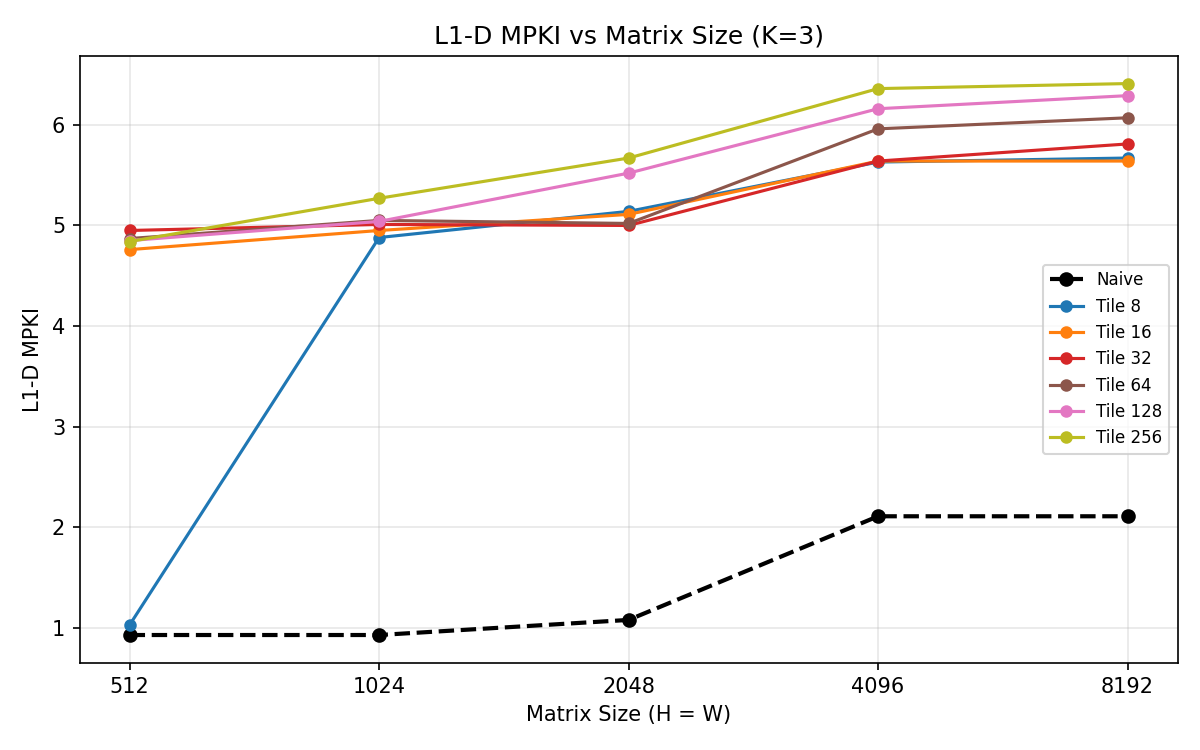
\includegraphics[width=0.8\textwidth]{../plots/tile_mpki_K3.png}
\caption{L1-D MPKI vs.\ Matrix Size for different tile sizes (K=3)}
\end{figure}

\begin{figure}[H]
\centering
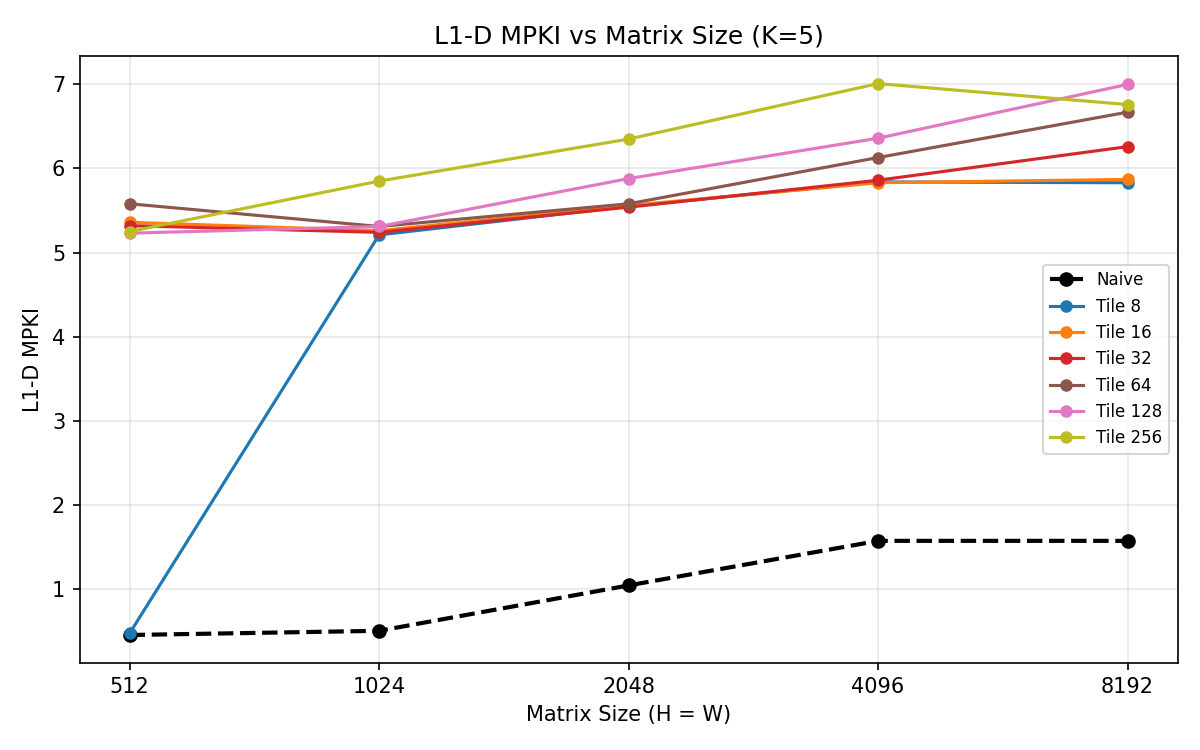
\includegraphics[width=0.8\textwidth]{../plots/tile_mpki_K5.png}
\caption{L1-D MPKI vs.\ Matrix Size for different tile sizes (K=5)}
\end{figure}

\subsubsection{Speedup vs.\ Matrix Size}

\begin{figure}[H]
\centering
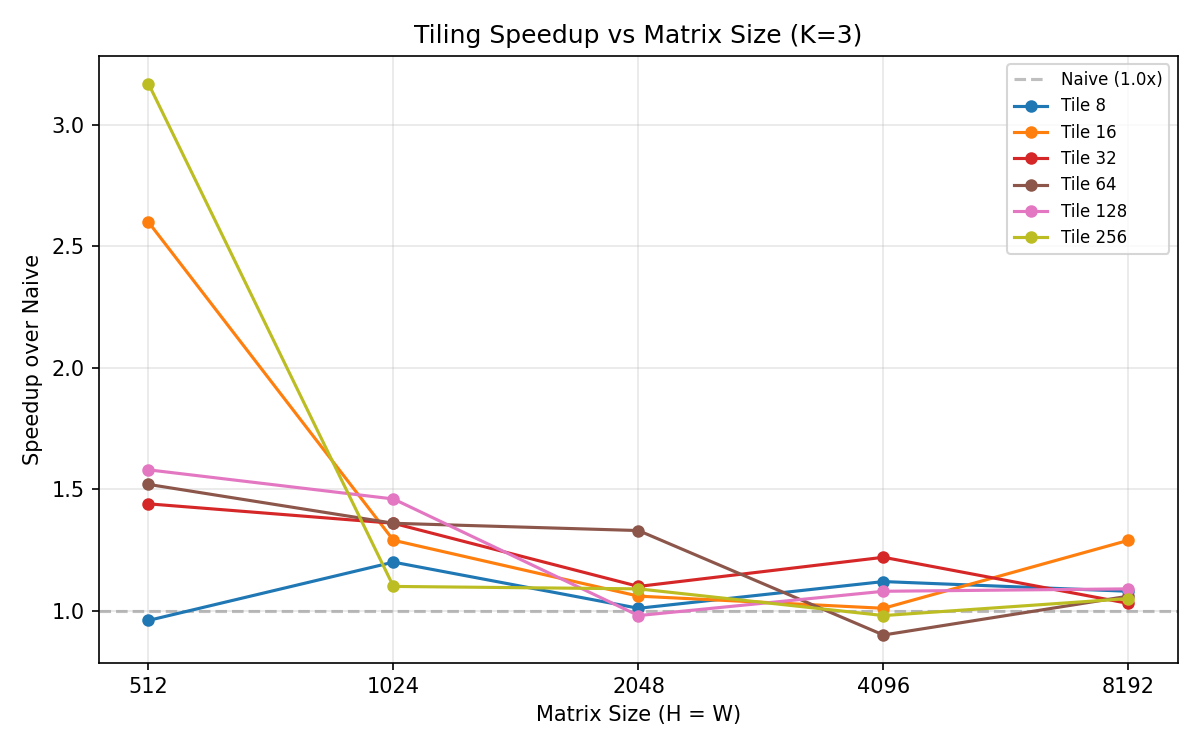
\includegraphics[width=0.8\textwidth]{../plots/tile_speedup_K3.png}
\caption{Speedup vs.\ Matrix Size for different tile sizes (K=3)}
\end{figure}

\begin{figure}[H]
\centering
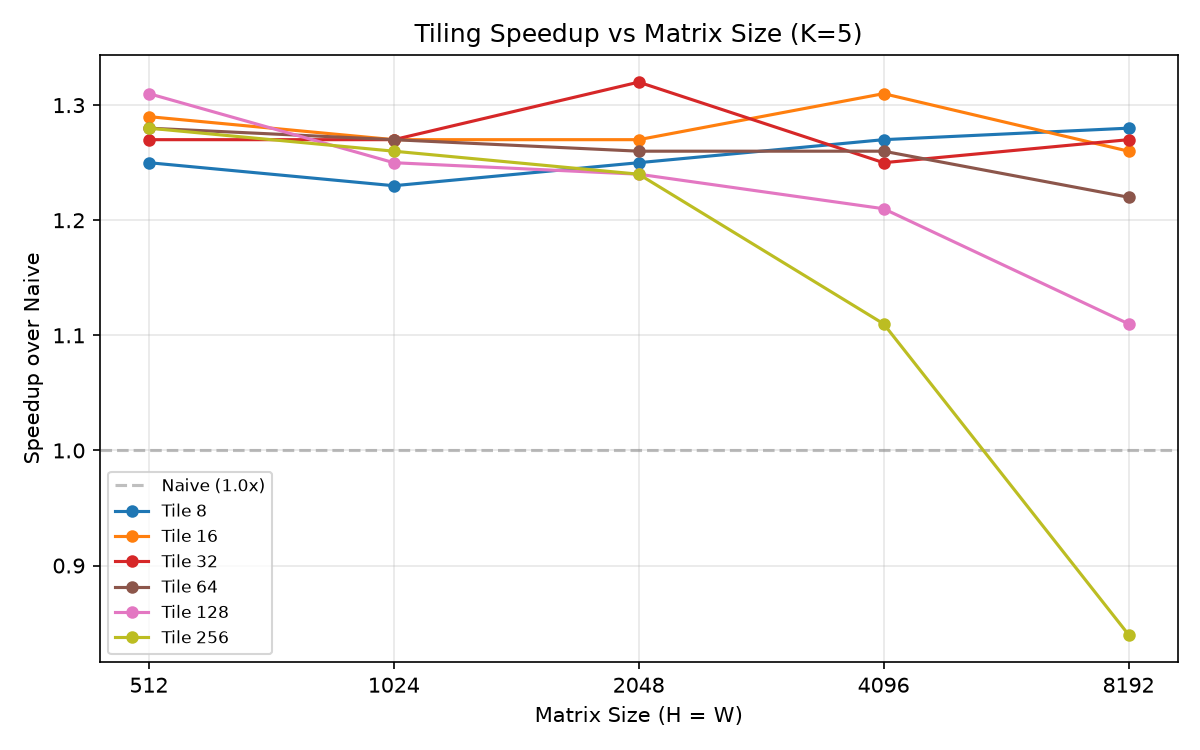
\includegraphics[width=0.8\textwidth]{../plots/tile_speedup_K5.png}
\caption{Speedup vs.\ Matrix Size for different tile sizes (K=5)}
\end{figure}

\subsection{Analysis Questions}

\subsubsection{Q1: Changes in L1-D MPKI from Naive to Tiled}

\todo{Report the changes in L1-D MPKI observed when moving from naive to
tiled 2D convolution. Justify your observations --- why does tiling
reduce (or not reduce) cache misses? Relate to the working set
fitting in L1.}

\subsubsection{Q2: How L1-D MPKI Varies Across Matrix Sizes and Tile Sizes}

\todo{Explain your findings in terms of the cache hierarchy and working set
sizes. For example: for small matrices, the entire output may fit in
cache even without tiling; for large matrices, smaller tiles keep the
strip in L1. Discuss the sweet spot.}

\subsubsection{Q3: Speedup Analysis}

\todo{Did you achieve a speedup? If yes, quantify the improvement and
identify the contributing factors (reduced cache misses, better
spatial locality). If not, analyze the limiting factors (e.g.\
overhead of zeroing, extra loop control) and propose possible
solutions.}

% ============================================================================
\section{Task 1C: SIMD (2 points)}
% ============================================================================

\subsection{Baseline Profiling}

\subsubsection{Instruction Count for Naive Implementation}

\begin{table}[H]
\centering
\caption{Naive convolution instruction count}
\begin{tabular}{lrr}
\toprule
Matrix Size & K=3 Instructions & K=5 Instructions \\
\midrule
512x512     & \naiveInsnsKthreeFtwelve & \naiveInsnsKfiveFtwelve \\
1024x1024   & \naiveInsnsKthreeTtwentyfour & \naiveInsnsKfiveTtwentyfour \\
2048x2048   & \naiveInsnsKthreeTfortyeight & \naiveInsnsKfiveTfortyeight \\
4096x4096   & \naiveInsnsKthreeFninetysix & \naiveInsnsKfiveFninetysix \\
8192x8192   & \naiveInsnsKthreeEonetwelve & \naiveInsnsKfiveEonetwelve \\
\bottomrule
\end{tabular}
\end{table}

\subsection{SIMD Implementation}

\subsubsection{128-bit (SSE)}

The 128-bit SSE implementation vectorizes the inner \texttt{ox} loop, processing 4 output pixels per iteration. The loop order is kept as the naive \texttt{oy, ox, ky, kx}. For each group of 4 output columns, a single \texttt{\_\_m128} accumulator is initialized to zero with \texttt{\_mm\_setzero\_ps()}. The kernel is then iterated over all $K \times K$ positions: at each position, the kernel weight is broadcast to all 4 lanes using \texttt{\_mm\_set1\_ps(ker[ky*K + kx])}, the 4 corresponding input values are loaded with \texttt{\_mm\_loadu\_ps(in\_row + kx)} (unaligned load, since input offsets are not guaranteed to be 16-byte aligned), and a fused multiply-add \texttt{\_mm\_fmadd\_ps(v, w, acc)} accumulates the products. After the full kernel has been applied, the result is written back with \texttt{\_mm\_storeu\_ps()}. A scalar tail loop handles the remaining $W \bmod 4$ columns per row.

\subsubsection{256-bit (AVX2)}

The 256-bit AVX2 implementation follows the same structure as SSE but processes 8 output pixels per iteration using 256-bit registers. The intrinsics used are the \texttt{\_mm256\_*} equivalents: \texttt{\_mm256\_setzero\_ps()} for initialization, \texttt{\_mm256\_set1\_ps()} for kernel weight broadcast, \texttt{\_mm256\_loadu\_ps()} for unaligned 8-float loads, \texttt{\_mm256\_fmadd\_ps()} for fused multiply-add, and \texttt{\_mm256\_storeu\_ps()} for the final store. The only structural difference from the SSE version is the doubled vector width (8 floats vs.\ 4), which halves the number of vector iterations over the output columns. A scalar tail loop handles the remaining $W \bmod 8$ columns.

\subsubsection{512-bit (AVX-512)}

AVX-512 \emph{is} available on the i5-11400H (\texttt{lscpu | grep avx512} reports
\texttt{avx512f}, \texttt{avx512dq}, \texttt{avx512bw} and \texttt{avx512vl}), so all
three widths --- 128-bit SSE, 256-bit AVX2 and 512-bit AVX-512 --- were measured. The
512-bit variant processes 16 floats per vector and is compiled with \texttt{-mavx512f};
the scalar optimisation level is unchanged from the pinned project flags so that only
the vector width differs between variants.

% [TODO: Discuss the 512-bit results. Note that the speedup is strongly size-dependent:
%  at K=3 AVX-512 reaches 12.32x at 512x512 but falls to 5.03x at 8192x8192, while at
%  K=5 it holds 11.5-12.6x across every size. Explain why (working set vs cache, and
%  the AVX-512 frequency/licence behaviour on this part).]

\subsection{Instruction Count for SIMD Implementations}

\begin{table}[H]
\centering
\caption{Instruction counts: naive vs.\ SIMD (K=3)}
\begin{tabular}{lrrr}
\toprule
Matrix Size & Naive & SSE 128-bit & AVX2 256-bit \\
\midrule
512x512     & \naiveInsnsKthreeFtwelve & \simdSSEKthreeFtwelveInsns & \simdAVXKthreeFtwelveInsns \\
1024x1024   & \naiveInsnsKthreeTtwentyfour & \simdSSEKthreeTtwentyfourInsns & \simdAVXKthreeTtwentyfourInsns \\
2048x2048   & \naiveInsnsKthreeTfortyeight & \simdSSEKthreeTfortyeightInsns & \simdAVXKthreeTfortyeightInsns \\
4096x4096   & \naiveInsnsKthreeFninetysix & \simdSSEKthreeFninetysixInsns & \simdAVXKthreeFninetysixInsns \\
8192x8192   & \naiveInsnsKthreeEonetwelve & \simdSSEKthreeEonetwelveInsns & \simdAVXKthreeEonetwelveInsns \\
\bottomrule
\end{tabular}
\end{table}

\begin{table}[H]
\centering
\caption{Instruction counts: naive vs.\ SIMD (K=5)}
\begin{tabular}{lrrr}
\toprule
Matrix Size & Naive & SSE 128-bit & AVX2 256-bit \\
\midrule
512x512     & \naiveInsnsKfiveFtwelve & \simdSSEKfiveFtwelveInsns & \simdAVXKfiveFtwelveInsns \\
1024x1024   & \naiveInsnsKfiveTtwentyfour & \simdSSEKfiveTtwentyfourInsns & \simdAVXKfiveTtwentyfourInsns \\
2048x2048   & \naiveInsnsKfiveTfortyeight & \simdSSEKfiveTfortyeightInsns & \simdAVXKfiveTfortyeightInsns \\
4096x4096   & \naiveInsnsKfiveFninetysix & \simdSSEKfiveFninetysixInsns & \simdAVXKfiveFninetysixInsns \\
8192x8192   & \naiveInsnsKfiveEonetwelve & \simdSSEKfiveEonetwelveInsns & \simdAVXKfiveEonetwelveInsns \\
\bottomrule
\end{tabular}
\end{table}

\subsection{Speedup Results}

\begin{table}[H]
\centering
\caption{SIMD speedups over naive (K=3)}
\begin{tabular}{lrr}
\toprule
Matrix Size & SSE 128-bit & AVX2 256-bit \\
\midrule
512x512     & \simdSSEKthreeFtwelveSpeedup & \simdAVXKthreeFtwelveSpeedup \\
1024x1024   & \simdSSEKthreeTtwentyfourSpeedup & \simdAVXKthreeTtwentyfourSpeedup \\
2048x2048   & \simdSSEKthreeTfortyeightSpeedup & \simdAVXKthreeTfortyeightSpeedup \\
4096x4096   & \simdSSEKthreeFninetysixSpeedup & \simdAVXKthreeFninetysixSpeedup \\
8192x8192   & \simdSSEKthreeEonetwelveSpeedup & \simdAVXKthreeEonetwelveSpeedup \\
\bottomrule
\end{tabular}
\end{table}

\begin{table}[H]
\centering
\caption{SIMD speedups over naive (K=5)}
\begin{tabular}{lrr}
\toprule
Matrix Size & SSE 128-bit & AVX2 256-bit \\
\midrule
512x512     & \simdSSEKfiveFtwelveSpeedup & \simdAVXKfiveFtwelveSpeedup \\
1024x1024   & \simdSSEKfiveTtwentyfourSpeedup & \simdAVXKfiveTtwentyfourSpeedup \\
2048x2048   & \simdSSEKfiveTfortyeightSpeedup & \simdAVXKfiveTfortyeightSpeedup \\
4096x4096   & \simdSSEKfiveFninetysixSpeedup & \simdAVXKfiveFninetysixSpeedup \\
8192x8192   & \simdSSEKfiveEonetwelveSpeedup & \simdAVXKfiveEonetwelveSpeedup \\
\bottomrule
\end{tabular}
\end{table}

\subsection{Plots}

\begin{figure}[H]
\centering
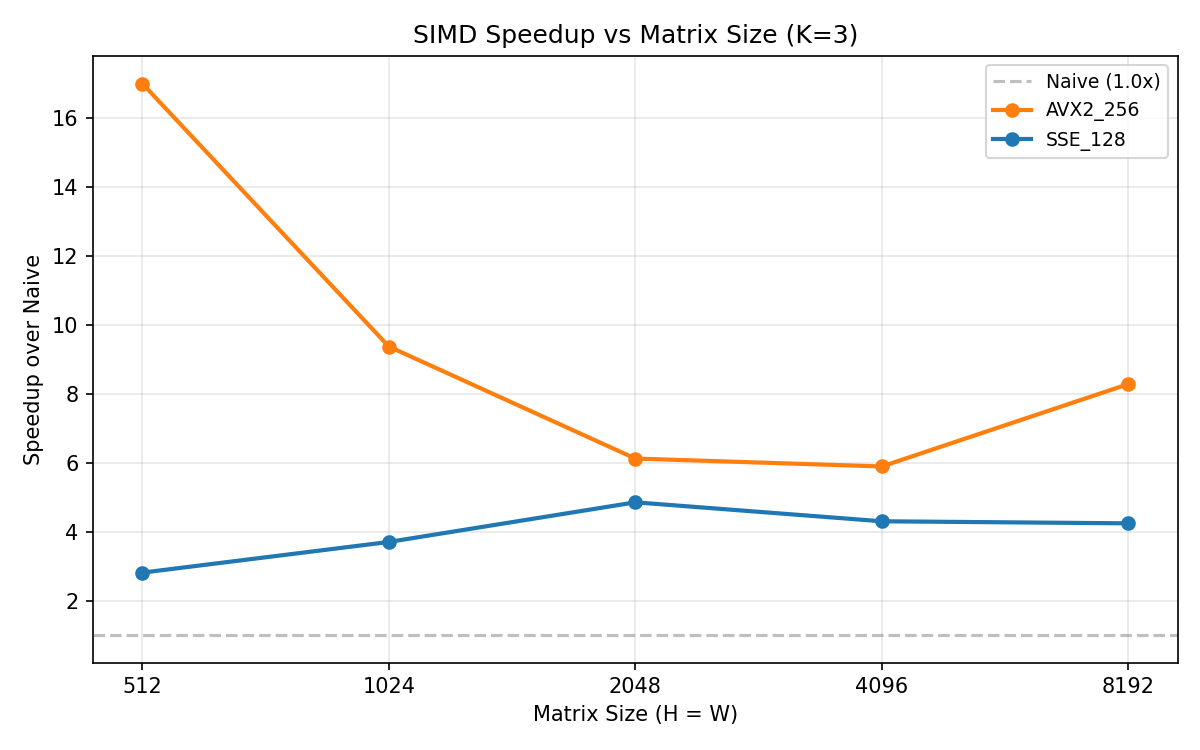
\includegraphics[width=0.8\textwidth]{../plots/simd_speedup_K3.png}
\caption{SIMD speedup vs.\ Matrix Size (K=3)}
\end{figure}

\begin{figure}[H]
\centering
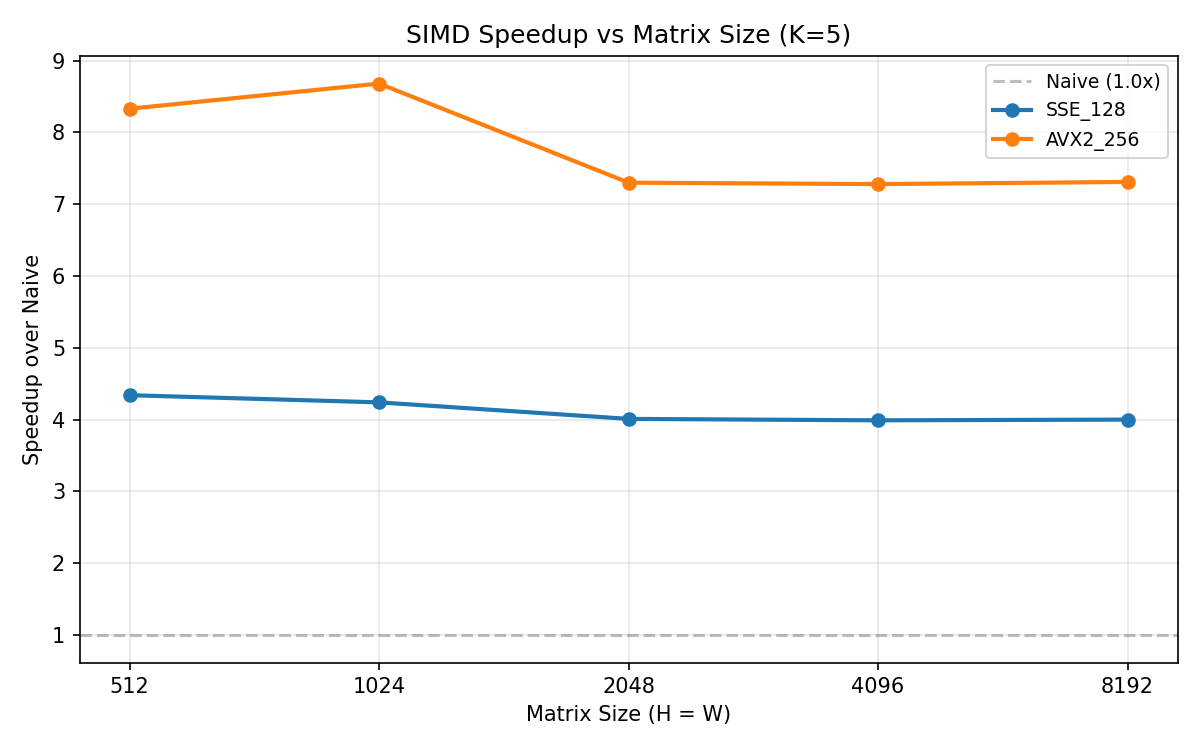
\includegraphics[width=0.8\textwidth]{../plots/simd_speedup_K5.png}
\caption{SIMD speedup vs.\ Matrix Size (K=5)}
\end{figure}

\subsection{Analysis Questions}

\subsubsection{Q1: Change in Instruction Count from Naive to SIMD}

\todo{Report the change in the number of instructions when moving from
naive to the SIMD implementation. Justify your observations ---
do instructions decrease? By how much? Is the reduction proportional
to the SIMD width (4x for SSE, 8x for AVX2)? If not, why?
(loop overhead, scalar remainder, setup instructions).}

\subsubsection{Q2: Speedup Analysis}

\todo{Did you achieve any speedup? If so, how much, and what contributed
to it? (reduced instruction count, better throughput per cycle,
FMA combining multiply+add). If not, what were the reasons?
(memory bandwidth bottleneck, cache misses dominating).}

\subsubsection{Q3: Choice of SIMD Intrinsics}

\todo{Which SIMD intrinsics did you use? Justify your choice of functions.
For example:
\begin{itemize}
    \item \texttt{\_mm256\_loadu\_ps}: unaligned load --- needed because
          input offsets are not always 32-byte aligned.
    \item \texttt{\_mm256\_set1\_ps}: broadcast kernel weight to all lanes.
    \item \texttt{\_mm256\_fmadd\_ps}: fused multiply-add --- combines
          multiply and add into a single instruction, reducing latency
          and instruction count.
    \item \texttt{\_mm256\_storeu\_ps}: unaligned store of result.
\end{itemize}}

% ============================================================================
\section{Task 1D: Sabka Saath Sabka Vikaas (2 points)}
% ============================================================================

\subsection{Combined Optimized Implementation}

\todo{Describe your combined implementation in \texttt{conv\_optimized.cpp}.
Which techniques did you combine? (e.g.\ SIMD + tiling, SIMD +
unrolling, SIMD + reordering, all of them). Explain how these
techniques complement each other for synergistic gains --- i.e.\
the combined benefit is greater than the sum of individual
optimizations.}

\subsection{Speedup Results}

\begin{table}[H]
\centering
\caption{Combined optimized speedup over naive}
\begin{tabular}{lrr}
\toprule
Matrix Size & K=3 Speedup & K=5 Speedup \\
\midrule
512x512     & \optimizedKthreeFtwelve & \optimizedKfiveFtwelve \\
1024x1024   & \optimizedKthreeTtwentyfour & \optimizedKfiveTtwentyfour \\
2048x2048   & \optimizedKthreeTfortyeight & \optimizedKfiveTfortyeight \\
4096x4096   & \optimizedKthreeFninetysix & \optimizedKfiveFninetysix \\
8192x8192   & \optimizedKthreeEonetwelve & \optimizedKfiveEonetwelve \\
\bottomrule
\end{tabular}
\end{table}

\subsection{Final Performance Summary Plot}

\begin{figure}[H]
\centering
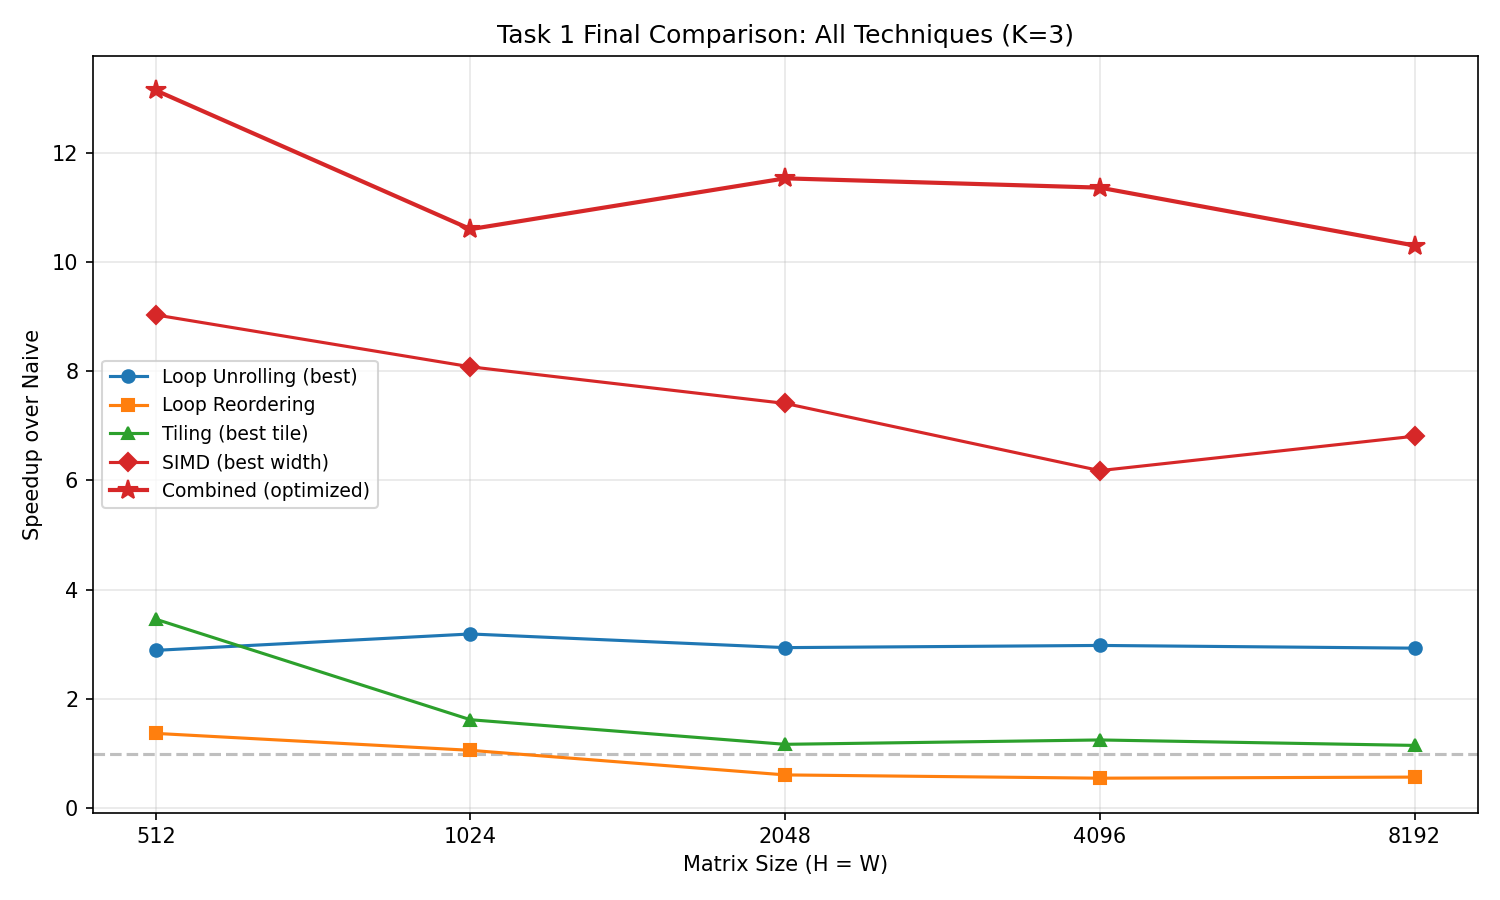
\includegraphics[width=0.8\textwidth]{../plots/final_comparison_K3.png}
\caption{Comparison of all optimization techniques --- Speedup vs.\ Matrix Size (K=3)}
\end{figure}

\begin{figure}[H]
\centering
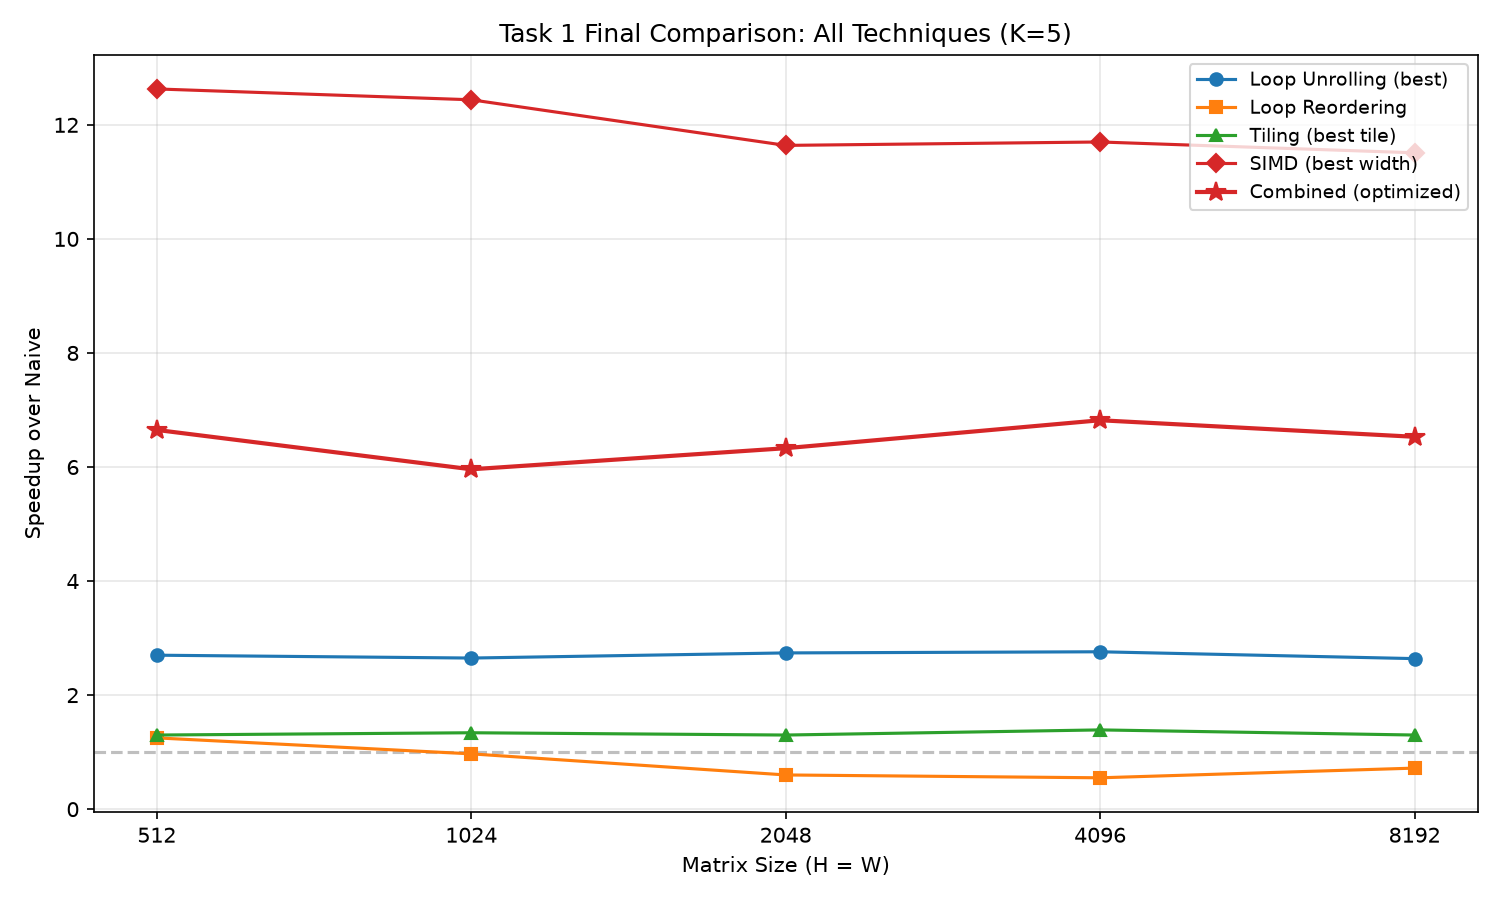
\includegraphics[width=0.8\textwidth]{../plots/final_comparison_K5.png}
\caption{Comparison of all optimization techniques --- Speedup vs.\ Matrix Size (K=5)}
\end{figure}

\subsection{Analysis}

\todo{Discuss how these techniques complement each other:
\begin{itemize}
    \item Why does combining techniques yield more than the sum of parts?
    \item Which combination gave the best speedup?
    \item What is the bottleneck of your best implementation?
          (compute-bound? memory-bound? Roofline analysis?)
    \item How does the gain/loss of each technique vary with matrix size
          and kernel size?
\end{itemize}}

% ============================================================================
% END
% ============================================================================

\end{document}
